%% abtex2-modelo-trabalho-academico.tex, v-1.9.1 laurocesar
%% Copyright 2012-2013 by abnTeX2 group at http://abntex2.googlecode.com/ 
%%
%% This work may be distributed and/or modified under the
%% conditions of the LaTeX Project Public License, either version 1.3
%% of this license or (at your option) any later version.
%% The latest version of this license is in
%%   http://www.latex-project.org/lppl.txt
%% and version 1.3 or later is part of all distributions of LaTeX
%% version 2005/12/01 or later.
%%
%% This work has the LPPL maintenance status `maintained'.
%% 
%% The Current Maintainer of this work is the abnTeX2 team, led
%% by Lauro César Araujo. Further information are available on 
%% http://abntex2.googlecode.com/
%%
%% This work consists of the files abntex2-modelo-trabalho-academico.tex,
%% abntex2-modelo-include-comandos and abntex2-modelo-references.bib
%%

% ------------------------------------------------------------------------
% ------------------------------------------------------------------------
% abnTeX2: Modelo de Trabalho Academico (tese de doutorado, dissertacao de
% mestrado e trabalhos monograficos em geral) em conformidade com 
% ABNT NBR 14724:2011: Informacao e documentacao - Trabalhos academicos -
% Apresentacao
% ------------------------------------------------------------------------
% ------------------------------------------------------------------------

\documentclass[
	% -- opções da classe memoir --
	12pt,				% tamanho da fonte
	openright,			% capítulos começam em pág ímpar (insere página vazia caso preciso)
	oneside,			% para impressão em verso e anverso. Oposto a oneside
	a4paper,			% tamanho do papel. 
	% -- opções da classe abntex2 --
	%chapter=TITLE,		% títulos de capítulos convertidos em letras maiúsculas
	%section=TITLE,		% títulos de seções convertidos em letras maiúsculas
	%subsection=TITLE,	% títulos de subseções convertidos em letras maiúsculas
	%subsubsection=TITLE,% títulos de subsubseções convertidos em letras maiúsculas
	% -- opções do pacote babel --
	english,			% idioma adicional para hifenização
	french,				% idioma adicional para hifenização
	spanish,			% idioma adicional para hifenização
	brazil				% o último idioma é o principal do documento
	]{abntex2}

% ---
% Pacotes básicos 
% ---
\usepackage{lmodern}			% Usa a fonte Latin Modern			
\usepackage[T1]{fontenc}		% Selecao de codigos de fonte.
\usepackage[utf8]{inputenc}		% Codificacao do documento (conversão automática dos acentos)
\usepackage{lastpage}			% Usado pela Ficha catalográfica
\usepackage{indentfirst}		% Indenta o primeiro parágrafo de cada seção.
\usepackage{color}				% Controle das cores
\usepackage{graphicx}			% Inclusão de gráficos
\usepackage{microtype} 			% para melhorias de justificação
\usepackage{enumitem}
\usepackage{eurosym}			% habilita símbolo do Euro

% ---
		
% ---
% Pacotes adicionais, usados apenas no âmbito do Modelo Canônico do abnteX2
% ---
\usepackage{lipsum}				% para geração de dummy text
% ---

% ---
% Pacotes de citações
% ---
\usepackage[brazilian,hyperpageref]{backref}	 % Paginas com as citações na bibl
\usepackage[alf]{abntex2cite}	% Citações padrão ABNT

% --- 
% CONFIGURAÇÕES DE PACOTES
% --- 

% ---
% Configurações do pacote backref
% Usado sem a opção hyperpageref de backref
\renewcommand{\backrefpagesname}{Citado na(s) página(s):~}
% Texto padrão antes do número das páginas
\renewcommand{\backref}{}
% Define os textos da citação
\renewcommand*{\backrefalt}[4]{
	\ifcase #1 %
		Nenhuma citação no texto.%
	\or
		Citado na página #2.%
	\else
		Citado #1 vezes nas páginas #2.%
	\fi}%
% ---

% ---
% Informações de dados para CAPA e FOLHA DE ROSTO
% ---
\titulo{CuboBrasil}
\autor{	Arnaldo Alves Viana Júnior - 09.01746-0\\
		Mayara Andressa Tezoni - 09.00697-4\\
		Maxwell da Silva Dias - 07.03287-0\\
		Otávio Moreira Petito - 08.01453-0\\
		Tiago Augusto Orcajo Demay Cordeiro - 09.02270-8\\
		Período: Noturno}
\local{São Caetano do Sul}
\data{2015}
\orientador{Prof. Me. Linduarte Vieira da Silva Filho}
%\coorientador{Professor}
\instituicao{Escola de Engenharia Mauá}
%tipotrabalho{Tese (Trabalho de Conclusão de Curso)}
% O preambulo deve conter o tipo do trabalho, o objetivo, 
% o nome da instituição e a área de concentração 
\preambulo{Trabalho de Gestão Empreendedora apresentado à Escola de Engenharia Mauá do Centro Universitário do Instituto Mauá de Tecnologia, como parte dos requisitos necessários à obtenção da aprovação da disciplina de Gestão Empreendedora Área de concentração: Engenharia Elétrica e Engenharia Química}
% ---


% ---
% Configurações de aparência do PDF final

% alterando o aspecto da cor azul
\definecolor{blue}{RGB}{41,5,195}

% informações do PDF
\makeatletter
\hypersetup{
     	%pagebackref=true,
		pdftitle={\@title}, 
		pdfauthor={\@author},
    	pdfsubject={\imprimirpreambulo},
	    pdfcreator={LaTeX with abnTeX2},
		pdfkeywords={abnt}{latex}{abntex}{abntex2}{trabalho acadêmico}, 
		colorlinks=true,       		% false: boxed links; true: colored links
    	linkcolor=black,          	% color of internal links
    	citecolor=black,        		% color of links to bibliography
    	filecolor=black,      		% color of file links
		urlcolor=black,
		bookmarksdepth=4 
}
\makeatother
% --- 

% --- 
% Espaçamentos entre linhas e parágrafos 
% --- 

% O tamanho do parágrafo é dado por:
\setlength{\parindent}{1.25cm}

% Controle do espaçamento entre um parágrafo e outro:
\setlength{\parskip}{0.2cm}  % tente também \onelineskip

% ---
% compila o indice
% ---
\makeindex
% ---

% ----
% Início do documento
% ----
\begin{document}

% Retira espaço extra obsoleto entre as frases.
\frenchspacing 

% ----------------------------------------------------------
% ELEMENTOS PRÉ-TEXTUAIS
% ----------------------------------------------------------
% \pretextual

% ---
% Capa
% ---
\imprimircapa
% ---

% ---
% Folha de rosto
% (o * indica que haverá a ficha bibliográfica)
% ---
\imprimirfolhaderosto*
% ---

% ---
% Inserir a ficha bibliografica
% ---

% Isto é um exemplo de Ficha Catalográfica, ou ``Dados internacionais de
% catalogação-na-publicação''. Você pode utilizar este modelo como referência. 
% Porém, provavelmente a biblioteca da sua universidade lhe fornecerá um PDF
% com a ficha catalográfica definitiva após a defesa do trabalho. Quando estiver
% com o documento, salve-o como PDF no diretório do seu projeto e substitua todo
% o conteúdo de implementação deste arquivo pelo comando abaixo:
%
% \begin{fichacatalografica}
%     \includepdf{fig_ficha_catalografica.pdf}
% \end{fichacatalografica}
\begin{fichacatalografica}
	\vspace*{\fill}					% Posição vertical
	\hrule							% Linha horizontal
	\begin{center}					% Minipage Centralizado
	\begin{minipage}[c]{12.5cm}		% Largura
	
	Júnior, Arnaldo Alves Viana
	
	\hspace{0.5cm} \imprimirtitulo  / Arnaldo Alves Viana Júnior, Otávio Moreira Petito e Tiago Augusto Orcajo Demay. --
	\imprimirlocal, CEUN-EEM, \imprimirdata
	
	\hspace{0.5cm} \pageref{LastPage} p. : il. \\
	
	\hspace{0.5cm}
	\parbox[t]{\textwidth}{\imprimirtipotrabalho~--~\imprimirinstituicao,
	\imprimirlocal, \imprimirdata.}\\
	
	\hspace{0.5cm} \imprimirorientadorRotulo~\imprimirorientador\\
	
	\hspace{0.5cm}
		1. Palavra-chave1.
		%2. Palavra-chave2.
		I. Tezoni, Mayara Andressa
		II. Dias, Maxwell da Silva
		III. Petito, Otávio Moreira
		IV. Cordeiro, Tiago Augusto Orcajo Demay
		V. Instituto Mauá de Tecnológia. Centro Universitário. Escola de Engenharia Mauá.
		VI. CuboBrasil\\ 			
	
	\hspace{8.75cm} CDU \\
	
	\end{minipage}
	\end{center}
	\hrule
\end{fichacatalografica}
% ---
\pagebreak



% ---
% inserir lista de ilustrações
% ---
\pdfbookmark[0]{\listfigurename}{lof}
\listoffigures*
\cleardoublepage
% ---

% ---
% inserir lista de tabelas
% ---
\pdfbookmark[0]{\listtablename}{lot}
\listoftables*
\cleardoublepage
% ---

% ---
% inserir lista de abreviaturas e siglas
% ---
%\begin{siglas}

%  \item[DPU] \textit{Data Processing Unit}
%  \item[CAN] \textit{Controller Area Network}
  
%\end{siglas}
% ---

% ---
% inserir lista de símbolos
% ---
%\begin{simbolos}
%  \item[$ \Gamma $] Letra grega Gama
%  \item[$ \Lambda $] Lambda
%  \item[$ \zeta $] Letra grega minúscula zeta
%  \item[$ \in $] Pertence
%\end{simbolos}
% ---

% ---
% inserir o sumario
% ---
\pdfbookmark[0]{\contentsname}{toc}
\tableofcontents*
\cleardoublepage
% ---

% ----------------------------------------------------------
% ELEMENTOS TEXTUAIS
% ----------------------------------------------------------
\textual



% ----------------------------------------------------------
% Introdução (exemplo de capítulo sem numeração, mas presente no Sumário)
% ----------------------------------------------------------
\chapter[Referência teórica]{Referência teórica}
	
	Segundo Philip Kotler (1992), o planejamento estratégico é uma metodologia gerencial que permite estabelecer a direção a ser seguida pela organização, visando maior grau de interação com o ambiente. O autor quando fala em direção, reforça sobre o âmbito de atuação, das macros políticas, macros objetivos, macro estratégia, das estratégias funcionais, políticas funcionais, objetivos funcionais e a filosofia de atuação da organização.
	
Sendo assim, o planejamento estratégico é uma ferramenta da administração que mapeia cenários futuros e gerencia informações vitais para a organização em um contexto competitivo, tornando-se o ponto chave para as criações de estratégias, sendo foco de atenção da alta administração organizacional.

O planejamento estratégico tem por objetivo desenvolver estratégias que guiarão a organização a obtenção de um melhor desempenho e, consequentemente, um melhor resultado. Existem vários modelos que são altamente eficazes e a organização deve identificar ou encontrar qual modelo que melhor se adapta a sua realidade.

O grau de interação entre o ambiente e a organização, pode ser positivo, negativo ou neutro. Pôde-se considerar como grau positivo as interações, ambiente-organização, que favorecem a organização. Já o grau negativo são todas as interações que trariam elementos nocivos à organização, e o grau neutro, que não traz nem beneficio e nem maleficio, é uma variável que fica na dependência de qualquer comportamento estratégico que a organização assumiu. Sendo assim, o planejamento estratégico estará sempre relacionado com o futuro da empresa e por meio desta ferramenta pode-se direcionar os elementos de crescimento à uma evolução lucrativa para os negócios.

Logo, o planejamento estratégico tem uma alta importância para o desenvolvimento da organização, pois é por meio dele que a organização pode determinar a melhor maneira de associar os recursos disponíveis com a necessidade do mercado, colocando em pratica as mudanças continuas que levem à maior produtividade e à melhor qualidade dos produtos e serviços. 

\section[Como montar um planejamento estratégico]{Como montar um planejamento estratégico}

\subsection[Definição dos itens para o planejamento estratégico]{Definição dos itens para o planejamento estratégico}

	Segundo Philip Kotler (1992), primeiramente, é necessário definir alguns itens de suma importância para o planejamento estratégico, como:
	
	\begin{enumerate}
		\item Os objetivos a serem atingidos por cada estratégia, preferencialmente de forma quantitativa;
		\item Como tais objetivos serão atingidos, quais as ações requeridas para que isto ocorra;
		\item Quais são os recursos necessários para implantar cada estratégia – Humanos, financeiros, tecnológicos etc;
		\item Os obstáculos a serem superados;
		\item As responsabilidades e prazos – quem fará o que e quando;
		\item O retorno esperado sobre o investimento.
	\end{enumerate}
		
	Caso contrário, não se tem um plano, mas apenas um desejo. E, o prazo do plano varia significamente de empresa para empresa. Ainda assim, normalmente desenham-se os cenários de mais longo prazo, procurando definir como o novo serviço ou produto estará competindo no mercado, que vantagens competitivas sustentáveis a tecnologia terá no futuro, mas fica muito difícil detalhar de forma concreta estratégias especificas de prazo mais longo. Assim, o plano será mais dinâmico e precisará ser revisado e renovado com maior frequência sempre que surgirem fatos novos importantes.
		
\subsection[Elaboração da estratégia]{Elaboração da estratégia}

	Logo depois da definição das diretrizes organizacionais, citadas no Item 2.1., a empresa necessita estabelecer os caminhos para alcança-las e esta é a finalidade da estratégica. Uma empresa voltada ao lucro compõe-se de um conjunto de ideias, praticas, processos e indivíduos que, associados e sustentandos por recursos sempre escassos, devem criar e capturar valor de forma superior a outras empresas que competem pelos mesmo clientes e necessidades.
	
	A elaboração da estratégia pode ser definida a quatro níveis:

	\begin{enumerate}
		\item Estratégia corporativa, que abrange toda a empresa e suas unidades de negócios;
		\item Estratégia de negócios, desenvolvida individualmente para as unidades de negócios que integram à corporação;
		\item Estratégia funcional, desenvolvida individualmente para os setores, por exemplo, estratégia de marketing e estratégia de produção, e
		\item Estratégia operacional, desenvolvida para regiões e unidades fabris específicas.
	\end{enumerate}
	
	Todas as esferas estratégicas desta estrutura são utilizadas por empresas diversificadas, porém, empresas menores, que trabalham somente em um negócio, utilizarão predominantemente as estratégias corporativa, de negócios e operacional.	
		
\subsection[Implementação da estratégia]{Implementação da estratégia}

	A implementação da estratégia consiste no momento mais importante de todo o processo, pois é nesta fase que o planejamento irá se concretizar. Atualmente, percebe-se que uma parcela mínima das estratégias formuladas são realmente implementadas. Em geral, os gestores buscam resolver esse problema, ampliando, o controle, buscando gerenciar a cultura organizacional ou ainda colocando a culpa nos executantes, alegando que esses são incapazes de colocar em prática o que foi formulado. Entretanto, o verdadeiro problema pode estar na separação entre formulação e implementação.
	
	Todavia, são poucos os administradores que percebem que um bom processo de planejamento estratégico também necessita um enfoque nos comos da execução da estratégia, deixando apenas de focar na elaboração (HREBINIACK, 2006). 
Conforme Bossidy e Charan (2002) estes comos da execução, abrangem todos os seus detalhes e devem nascer na mente das pessoas que estão mais próximas da ação e que necessariamente entendem seus mercados, seus recursos e seus pontos fortes e fracos, diferentemente, ela será um fracasso.

	Entretanto, Bossidy e Charan (2002) enfatizam que pensar na execução somente como o sentido tático do planejamento estratégico, como alguma coisa que os líderes consideram como “mais importantes”, está muito errado, pois executar não é simplesmente uma tática, é uma disciplina, um sistema, que deve estar introduzida na estratégia da empresa, em seus objetivos e em sua cultura, contando sempre com um líder intensamente envolvido com a implementação. 
	
	Brenes et al (apud Kich e Pereira, 2011) pensam da mesma forma que Bossidy e Charan (2002), quando asseguram que a implementação de uma estratégia de sucesso não é somente um aglomerado de “iniciativas estratégicas” e atividades relacionadas a ela, que são desenvolvidas por distintas pessoas. Pelo contrário, a implementação da estratégia, deve ser verificada como a construção de uma vantagem competitiva, de forma consciente e coordenada, por meio do gerenciamento dos vários componentes organizacionais, tanto de dentro, quanto de fora da empresa. Os mesmos afirmam que a execução da estratégia e o sucesso na sua aplicação são determinados pelo grau de alinhamento entre estrutura e cultura organizacional, a capacidade de efetivamente delegar responsabilidades, bem como o alinhamento entre os processos, os sistemas de trabalho, e os sistemas de informação.
	
	Desta forma, Bossidy (2002) defende que a maior causa do fracasso das empresas, é a incapacidade destas de executarem suas idéias e estratégias, pois falta disciplina para criar, promover e executar um sistema integrado, que envolva as pessoas, a estratégia e as operações da organização. Diante disto, Oliveira (apud Kich e Pereira, 2011) afirma que a qualidade da implementação das estratégias empresariais é resultante de três vertentes: qualidade na formulação das estratégias; qualidade na escolha das estratégias básicas; e qualidade decisória e administrativa da equipe que cataliza e ordena a implementação das estratégias. 
	
	Bossidy e Charan (2002) partilha desta mesma idéia ao garantirem que as estratégias, na maioria das vezes, não dão certo porque não foram bem executadas e que as coisas que deveriam acontecer não aconteceram porque as organizações não foram capazes de fazer com que elas acontecessem, ou mesmos líderes analisaram mal os desafios que as empresas confrontariam na momento dos negócios, ou ambos. 
	
	No entanto, é necessário que os administradores entendam que a elaboração e a implementação da estratégia são interdependentes. Neste sentido, Bossidy e Charan (2002, p.178) afirmam que “um bom processo estratégico é umas das melhores formas de ensinar as pessoas sobre execução”. 
	
	Mintzberg (1998) entende dessa mesma forma, porque assegura que na maioria das vezes que uma estratégia não é realizada, a culpa é depositada na implementação, enquanto, segundo ele, dever-se-ia ir além e procurar a causa na formulação dela, pois os gerentes que deveriam ter sido mais inteligentes, fazendo com que suas estratégias se desenvolvessem gradualmente, por meio das ações e experiências da organização. Por isso, o autor defende com convicção o uso das chamadas “estratégias emergentes”, que são aquelas que se originam durante a implementação do planejamento estratégico, ou seja, as estratégias que não foram previamente elaboradas.
	
\section[Plano de marketing]{Plano de marketing}

	Segundo Pereira (2011), um Plano de Marketing é um documento que detalha as ações necessárias para atingir um ou mais objetivos de marketing, adaptando-se a mudanças e identificando tendências. Esta ferramenta pode cobrir entre um e cinco anos de uma empresa ou negócio, sendo muito importante a sua atualização. O planejamento pode ser feito para a marca, para um produto ou serviço, ou para as linhas de produtos. O Plano de Marketing deve ser entendido como um complemento ao Plano de negócios e como um instrumento indispensável ao desenvolvimento da empresa. Por linhas gerais, ao realizar um Plano de Marketing, primeiro deve-se fazer um planejamento iniciado por uma Análise de Mercado, levantando dados como a realidade da sua empresa, dos seus produtos, dos seus mercados e da concorrência. Ao sistematizar essas informações, já será possível identificar as ameaças e as oportunidades, potenciais ou reais, que vão determinar toda a execução das estratégias. O segundo passo é a formulação das estratégias, que terão como objetivo aproveitar as oportunidades e contornar as ameaças. Em seguida, dá-se início à prática, definindo-se o próprio Plano de Marketing.
	
\subsection[As atividades de marketing]{As atividades de marketing}

	Para Pereira (2011), um profissional de Marketing é responsável pelo planejamento, pela organização e pelo controle das atividades estratégicas e táticas de marketing, na busca de aperfeiçoar e desenvolver valor para o cliente.
	
	Pode-se dizer que os 4 A’s do marketing estão relacionados com a Inteligência Competitiva, pois serão utilizados para buscas de informações estratégicas externamente, ou seja, em seus concorrentes. Além da Inteligência Competitiva será de tamanha importância a Pesquisa de Mercado, pois com ela obtêm-se as informações necessárias para suprir os 4 A’s, que são:
	
	\begin{enumerate}
		\item \textbf{Análise}: Visa identificar as forças vigentes no mercado e suas interações com a empresa. Os meios utilizados para tal fim são: pesquisa de mercado e o sistema de informação em marketing;
		\item \textbf{Adaptação}: É o processo de adequação das linhas de produtos ou serviços da empresa ao meio ambiente identificado através da análise. E isso ocorre através da apresentação ou configuração básica do produto: design, embalagem ou marca. E ainda por meio do preço e da assistência ao cliente;
		\item \textbf{Ativação}: Os elementos chave da ativação são a distribuição (seleção dos canais), a logística (entrega e armazenamento de produtos), a venda de pessoal (esforço para efetuar a transferência de posse do bem ou serviço) eo composto de comunicação (publicidade, promoção de vendas, relações públicas e merchandising);
		\item \textbf{Avaliação}: É o controle dos resultados do esforço de marketing, isoladamente e em conjunto. Essa função também é chamada de Auditoria de Marketing.
	\end{enumerate}

\subsection[Finalidades básicas do marketing]{Finalidades básicas do marketing}
	
	As funções do marketing incluem, basicamente, cinco partes que são compreender o mercado, conhecer os cliente em potêncial de modo que nichos e segmentos de mercado possam ser identificados e escolhidos (Pereira, 2011).
	
	Programas de marketing são criados, planejados, executados e controlados para que estas funções sejam executadas, antes da execução é necessário preparar a organização (conjunturalmente) para que as atividades de marketing sejam executadas com sucesso.
	
\subsection[Os 4 P's de marketing]{Os 4 P's de marketing}

	As estratégias de marketing é o caminho pelo qual você chegará a suas metas e objetivos. Ainda por meio delas, será possível encontrar maneiras de obter vantagens sobre os seus concorrentes. É nesta parte do Plano de Marketing que você vai definir quais ações deverão ser realizadas para o sucesso de seu negócio. As estratégias de marketing estão intimamente ligadas aos 4 P’s de Marketing (Produto, Preço, Praça e Promoção ). São eles que define como estes itens estarão relacionados.

	\begin{enumerate}
		\item \textbf{Produto}: O produto pode ser classificado como tangível, como um objeto, ou intangível, como um serviço. O produto é o bem ofertado nas transações comerciais e deve proporcionar aquele que o compra, benefícios e vantagens, além de satisfazer suas necessidades básicas. Para tornar um produto mais atrativo, você pode oferecer embalagens diferenciadas, garantia, entrega gratuita, etc. Todo produto possui um ciclo de vida. Ele é composto pelas seguintes fases: germinação, crescimento, maturação, declínio e morte. A cada uma dessas fases, deve-se aplicar uma estratégia diferente. Na germinação, ou seja, no surgimento do produto, o lucro com as vendas é baixo, já que as pessoas ainda estão se conscientizando sobre a utilidade daquele produto. Vale investir em divulgação e algum tipo de propaganda. No crescimento, o mais apropriado é que você busque manter a fidelidade dos clientes e uma boa relação com eles. Dessa forma, o crescimento das vendas é assegurado. Na maturação, quando o mercado daquele produto está começando a se saturar e surgem cada vez mais concorrentes, o ideal é fortalecer ainda mais as relações com o cliente. Para isso, descontos especiais, cartão fidelidade, dentre outras medidas, são opções indicadas. Entretanto, quando esta fase vai chegando ao fim, é o momento de buscar algum tipo de inovação, seja encontrando novas utilidades ao seu produto ou tentando criar outros produtos atrativos para o sue mercado. Na fase de declínio e morte, outros produtos com mais benefícios e vantagens comparativas poderão substituir o seu. Campanhas de marketing muitas vezes não se mostram tão eficazes neste estágio, mas a fidelidade do cliente (note que ela está presente em quase todas as fases) e o marketing “boca-a-boca” devem ser trabalhados com atenção. Exemplificando, o celular é um tipo de produto que vem sendo usado há quase 20 anos e ainda não encontrou um substituto perfeito. Entretanto, para que as empresas que o produziam não perdessem mercado, elas inovaram e deixaram o celular muito mais funcional, com câmera, mp3, internet. Enfim, estas empresas buscaram ideias para suprir as necessidades diferenciadas de seus clientes.
		\item \textbf{Preço}: Preço é o valor em dinheiro que seu produto vale para o consumidor. O preço precisa ser suficiente para cobrir os custos de produção e ainda trazer algum lucro para o dono do empreendimento. Definido o preço ideal para o produto, basta verificar se está compatível com o quanto o consumidor deseja pagar e com o mercado atual. A fixação do preço é crucial para a definição de fatores como o posicionamento do negócio, além de ser intimamente ligado às metas da empresa. Os preços de um mesmo produto podem variar de acordo com a sazonalidade, períodos promocionais, regiões, descontos etc. Você também não deve se esquecer de comparar os seus preços aos da concorrência.
		\item \textbf{Praça}: Este item é o que define a forma como o produto será disponibilizado ao cliente, levando em consideração a localização, os canais de distribuição e relação com os fornecedores. Antes de escolher o tipo de canal que mais o favoreça, observe as características dos possíveis fornecedores, transporte necessário, operacionalização de seu produto, estoques. A localização também dependerá do seu tipo de negócio. Analise a relação custo x benefício e escolha uma localização que contribuirá com o seu negócio, como boa visibilidade, fácil acesso, estrutura adequada, estacionamento, entre outros aspectos. Invista em uma boa estrutura para deixar seu cliente à vontade: vitrines atrativas, boa iluminação, boa disposição dos produtos, sinalização, etc.
		\item \textbf{Promoção}: A promoção possui três objetivos: Informar aos clientes potenciais a existência dos produtos e serviços e de suas vantagens; informar aos clientes potenciais onde e como obter esses serviços; lembrar aos clientes a existência dos produtos e serviços oferecidos. Os meios de comunicação escolhidos devem ser os de preferência dos seus clientes e lembre- se de direcionar o anúncio ao público certo. A internet pode ser uma ferramenta institucional, ou seja, uma ferramenta que permite ao consumidor acessar e conhecer a estrutura do negócio, os produtos vendidos, além de informações como telefone e localização. A Comunicação no ponto de venda diz respeito a toda a sinalização – displays, cartazes e outras variedades de materiais visuais que influenciam a decisão de compra. Tenha em mente quem é o seu público e saiba quais os principais meios que ele utiliza, pois a escolha dos meios de comunicação será ditada pelas necessidades e comportamento do consumidor.
	\end{enumerate}

\section[Análise do plano de marketing]{Análise do plano de marketing}

\subsection[Análise do mercado]{Análise do mercado}

	\begin{enumerate}
		\item \textbf{Analisar o ambiente de marketing}
		
		O primeiro passo é avaliar quais são os fatores externos e internos que podem influenciar a sua pequena empresa. “Além disso, é preciso analisar o segmento e o produto e ver quais são as capacidades do negócio”, explica Altaffer.
			
		Para ele, é imprescindível que o empreendedor tenha humildade para colocar no papel quais são as suas forças e fraquezas, e o capital disponível que poderá ser usado nas ações de marketing, pois caso contrário, o plano não terá sustentabilidade a longo prazo.
		\pagebreak
		\item \textbf{Entender quem são os seus clientes}
		
		Às vezes, o público alvo de sua empresa não é o consumidor. O público alvo de uma determinada marca de leite achocolatado, por exemplo, são as crianças, ainda que ela tenha um número grande de consumidores adultos. “Um plano de marketing tem que ser voltado para o público alvo”, diz Bedendo (2012).
		
		Analisar o mercado também é importante, prestando atenção nas demandas, no potencial, na previsão de taxa de crescimento e de participação. De acordo com Altaffer (2012), é preciso também entender como, por que e quando os consumidores usam o seu produto ou serviço. “A melhor pesquisa de mercado é a conversa do balcão; não pode é ter medo de perguntar”, ensina ele.
		
		\item \textbf{Analisar os concorrentes}
		
		Avalie de maneira detalhada quem são e quais são os objetivos dos principais players de seu mercado. “É importante também olhar para outras empresas do setor que possa entregar os mesmos benefícios que a sua empresa”, recomenda Altaffer.
		
		\item \textbf{Definir suas estratégias e ações}
		
		Primeiramente, é necessário estabelecer o objetivo do plano. Por exemplo, se o empreendedor deseja aumentar o número de vendas, ele precisa entender de onde vem o faturamento de suas vendas e avaliar se o ideal é fazer com que os clientes comprem com mais frequência ou se a chave é buscar novos consumidores.
		
		Em seguida, é hora de avaliar quais medidas serão adotadas pela empresa. Para os especialistas, utilizar as redes sociais, dar desconto no mês de aniversário do cliente são alguns exemplos de ações.
		
		\item \textbf{Estabelecer um cronograma}
		
		O monitoramento da duração de cada ação, os resultados e os recursos necessários que foram utilizados devem ser colocados no papel. “Quando você não tem isso registrado, fica difícil avaliar o que deu certo”, explica Bedendo.
		
	Para Altaffer, todo plano de marketing não tem fim, pois é recomendável que este seja revisado, refeito e atualizado com dados como número de vendas, faturamento, rentabilidade, entre outros.
		
	\end{enumerate}

\subsection[Estratégia de marketing]{Estratégia de marketing}

	Estratégia é a produção de planos para atingir objetivos. Estratégias de Marketing são aqueles planos desenhados para atingir objetivos do marketing. Uma boa estratégia de marketing deveria integrar os objetivos, políticas, e sequências de ação (tática) num todo coerente da organização. O objetivo de uma estratégia de marketing é colocar a organização numa posição de cumprir eficientemente a sua missão.
	
\section{Regime tributário}

	Para  fins tributários federais, a apuração dos impostos, no Brasil, pode ser feita de três formas:
	
	\begin{enumerate}
		\item Lucro real;
		\item Lucro presumido;
		\item Simples nacional.
	\end{enumerate}
	
\subsection{Lucro Real}

	No Lucro Real, o imposto de renda e a contribuição social sobre o lucro são determinados a partir do lucro contábil, apurado pela pessoa jurídica, acrescido de ajustes (positivos e negativos) requeridos pela legislação fiscal. Também neste regime o PIS e COFINS são determinados (com exceções específicas) através do regime não cumulativo, creditando-se valores das aquisições realizadas de acordo com os parâmetros e limites legais.
	
\subsection{Lucro presumido}

	No Lucro Presumido realiza-se a tributação simplificada do Imposto de Renda das Pessoas Jurídicas (IRPJ) e Contribuição Social sobre o Lucro (CSLL). Entretanto, no Lucro Presumido, o limite da receita bruta para poder optar, a partir de 2014, é de até R\$ 78 milhões da receita bruta total, no ano-calendário anterior. Outro detalhe é que as empresas tributadas pelo Lucro Presumido não podem aproveitar os créditos do PIS e da COFINS, por estarem fora do sistema não cumulativo, no entanto recolhem tais contribuições com alíquotas mais baixas do que aquelas exigidas pelo Lucro Real.

\subsection{Simples nacional}

	No regime tributário conhecido como Simples Nacional, há normas simplificadas no cálculo e recolhimento de tributos (IRPJ, CSLL, PIS, COFINS, IPI, Contribuições Previdenciárias, alcançando também o ICMS e o ISS) das microempresas e empresas de pequeno porte. Nem todas empresas podem optar pelo Simples, a primeira barreira é em relação à receita bruta anual, que deve restringir-se ao teto de R\$ 3.600.000 anuais (valor vigente para opção em 2013). 
	
Determinadas atividades ou formas societárias estão vedadas de adotar o Super Simples – dentre essas vedações, destacam-se:
	\begin{enumerate}
		\item pessoas jurídicas constituídas como cooperativas (exceto as de consumo);
		\item empresas cujo capital participe outra pessoa jurídica;
		\item pessoas jurídicas cujo sócio ou titular seja administrador ou equiparado de outra pessoa jurídica com fins lucrativos, desde que a receita bruta global ultrapasse o limite de receita.
	\end{enumerate}

Ficaram fora da vedação ao regime, as empresas de serviços contábeis, que poderão ser optantes pelo Simples Nacional.

\chapter[A empresa]{A empresa}

	Atualmente o mercado aeroespacial encontra-se em expansão devido aos \textit{CubeSats} que desenvolvidos, possuem alto poder de processamento e com um custo relativamente baixo comparado aos satélites tradicionais. Aproveitando o 'boom' aeroespacial, a CuboBrasil chega com a finalidade de aproximar essa tecnologia ao mercado latino americano, que possuem uma grande carência de fabricantes dessa tecnologia.
	
	A CuboBrasil é uma empresa especializada no mercado aeroespacial e comercializa satélites miniatuarizados conhecidos como \textit{CubeSats}. 
	
	Foi fundada no inicio de 2015 por alunos de Engenharia da Escola de Engenharia Mauá do Instituto Mauá de Técnologia (IMT-EEM). 
	
	Seu \textit{business chain} é focado no além das vendas dos satélites e subsistemas, mas também de serviços que agreguem valor ao produto final que é o \textit{CubeSat}. Pelo seu \textit{know-how} diferenciado no mercado aeroespacial, a CuboBrasil presta serviços como: treinamento/curso, consultoria e manutenção. Destaca-se como potencial desta empresa o fato do pioneirismo à pesquisa e desenvolvimento da tecnologia nacional associada ao compromisso de custo/benefício. O mercado potencial são instituições de ensino e/ou pesquisa, defesa militar e hobistas.
	
	Um \textit{CubeSat} (acrônimo das palavras em inglês: \textit{Cube} e \textit{Satellite} - Cubo e Satélite) é um tipo de satélite miniaturizado usado para pesquisas espaciais e comunicações radioamadoras. Os \textit{CubeSats} normalmente possuem volume de 1 litro (um cubo de 10 cm) e massa de até 1,33 kg. Normalmente, esse tipo de satélite usa componentes eletrônicos "de prateleira".
	
	O termo "\textit{CubeSat}" foi criado para designar nanossatélites que estão de acordo com o padrão descrito na especificação do \textit{CubeSat}. A "\textit{Cal Poly}" publicou o padrão como resultado de um projeto liderado pelo professor de engenharia aeroespacial Jordi Puig-Suari. Bob Twiggs, do Departamento de Aeronáutica e Astronáutica da Universidade de Stanford, e atualmente membro da faculdade de ciências espaciais na Morehead State University no Kentucky, tem contribuído com a comunidade \textit{CubeSat}. Seus esforços tem se concentrado em \textit{CubeSats} de instituições educacionais. A especificação não se aplica a outros satélites em formato de cubo tais como a do nanossatélite "MEPSI" da NASA, que é maior que um \textit{CubeSat}.

	Já em 2004, com o seu tamanho relativamente pequeno, os \textit{CubeSats} podiam ser construídos e lançados por um custo estimado de \$65.000 a \$80.000. Esse custo, muito menor que o de satélites "convencionais", fez do \textit{CubeSat} uma opção viável para escolas e universidades ao redor do mundo. Por conta disso, um grande número de universidades, algumas empresas e até mesmo instituições governamentais, passaram a desenvolver \textit{CubeSats}.
	
	No Brasil essa tecnologia é recente e escassa, sendo assim uma área a ser desenvolvida e consolidada nacionalmente, isto pelo fato de possuir custo elevado e requerer tempo dedicado à pesquisa de novas tecnologias.
A empresa vem com o \textit{know-how}, plataforma e condições necessárias para sanar a carência que o mercado nacional possui no setor aeroespacial, oferecendo tecnologia de ponta, novos conceitos, facilidades de acesso a seus produtos.

\section[Missão]{Missão}
	
	Oferecer alta tecnologia para promover e fomentar o desenvolvimento no setor aeroespacial, facilitar o acesso a instituições e grupos de pesquisa e universidades fortalecendo o interesse nas atividades espaciais brasileiras. Visando cada vez mais expandir nosso mercado.
	
\section[Visão]{Visão}	
	
	Ser a empresa brasileira pioneira no desenvolvimento do setor aeroespacial, tornando-se referência nacional de qualidade e tecnologia.
	
\section[Valores]{Valores}

	Cooperativismo, honestidade, novas ideias, responsabilidade social, acessibilidade, ética.

\section[Estrutura Organizacional]{Estrutura Organizacional}

	A estrutura organizacional é um elemento importantíssimo para manter o foco nos objetivos da empresa, depois da definição da missão, visão e valores.	
	
	A estrutura organizacional da CuboBrasil, inicialmente, será muito simples. Essa simplicidade deve-se ao fato da CuboBrasil ser uma microempresa que estará entrando em um segmento de mercado extremamente desafiador, onde os valores vinculados aos produtos são elevados e os produtos não possuem grande liquidez.
	
	Uma estrutura simplificada irá auxiliar no controle dos custos internos da empresa, visando maximizar o lucro e potencializar as vendas.
	
	\begin{figure}[th]
		\caption{ORGANOGRAMA DA CUBOBRASIL}
		\centering
		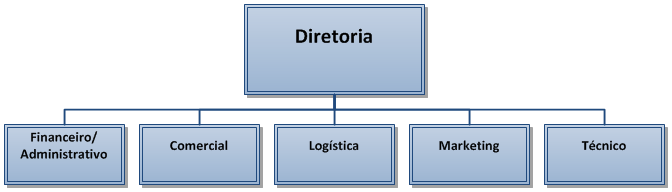
\includegraphics[width=1.0\linewidth]{./figs/Figura_10}
		
		\begin{small}
			FONTE: Elaborado pelos autores.
		\end{small}
	\end{figure}
	\pagebreak
	Na estrutura definida, a atuação dos empreendedores é fundamental. A divisão entre os 5 departamentos foi realizada de forma onda cada um dos sócios possam atuar. Importante ressaltar que cada um dos empreendedores estará atuando de forma ativa e sempre embasados nos conhecimentos adquiridos em cursos e pesquisas, visando dessa forma alcançar os melhores resultados possíveis de maneira consciente.
	
\chapter[Plano de marketing e vendas]{Plano de marketing e vendas}

	O plano de marketing é algo essencial para o planejamento do negócio, pois ele garantirá que os objetivos de marketing serão atingidos, adaptando-se as mudanças e identificando as tendências do mercado. Além de que, o plano de marketing pode assegurar que a empresa será coberta entre um e cinco anos, sendo essencial a atualização dos dados contidos nele. 

\section[Caracterização e análise do mercado]{Caracterização e análise do mercado}

	O mercado aeroespacial está em fase de “decolagem” no Brasil, conforme demonstrado na Figura 1, com apoio de diversas empresas (como a Embraer) e dos governantes dos principais estados do país focados em ganhar o espaço, o estado de São Paulo por exemplo concentra atualmente o maior polo aeroespacial da América Latina.

	\begin{figure}[th]
		\caption{RECEITA DAS INDÚSTRIAS AEROESPACIAIS DO BRASIL}
		\centering
		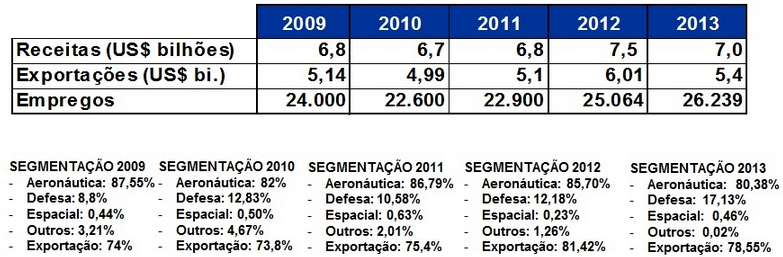
\includegraphics[width=0.8\linewidth]{./figs/Figura_01a}
			
		\begin{small}
			FONTE: Associação das Indústrias Aeroespaciais do Brasil
		\end{small}		
	\end{figure}

	Os números de mercado em nível mundial na indústria de satélites movimentam da ordem de US\$ 50 bilhões por ano. 
No Brasil movimentam algo em torno de US\$ 550 milhões por ano, liderança no Brasil, STAR ONE detém mais de 50 \% de “\textit{market share}”.

	Segundo Antônio Bertachini Prado, doutor em engenharia espacial e coordenador dos cursos de pós-graduação do Instituto Nacional de Pesquisas Espaciais (Inpe), o mercado é bastante promissor para profissionais que se especializam no planejamento e na execução de lançamento de veículos espaciais, como satélites e foguetes. “No entanto, a oferta de profissionais ficará pequena com o passar dos anos. A maioria dos profissionais que atuam nessa área hoje é de matemáticos, físicos e engenheiros com mestrado ou doutorado em aeroespacial. Faltam cursos que preparem e orientem desde cedo”, comenta. Ele explica que o Inpe prevê, para os próximos 10 anos, o aumento gradativo das missões espaciais.
		
	Assim os Institutos de Pesquisa e as universidades necessitam cada vez mais de acesso a alta tecnologia crescimento que garante a carência pelos \textit{CubeSats}.
		
	Na América Latina, principalmente no Brasil, existe uma grande oportunidade para entrar no mercado, uma vez que poucas empresas atuam diretamente com essa região. No Brasil, atualmente, não existem empresas focadas no mercado de satélites e por consequência dos \textit{CubeSats}, como é possível verificar na Associação das Indústrias Aeroespaciais do Brasil.
	
	\begin{figure}[th]
		\caption{SEGMENTAÇÃO DAS EMPRESAS AEROESPACIAIS BRASILEIRAS}
		\label{Segmentação}
		\centering
		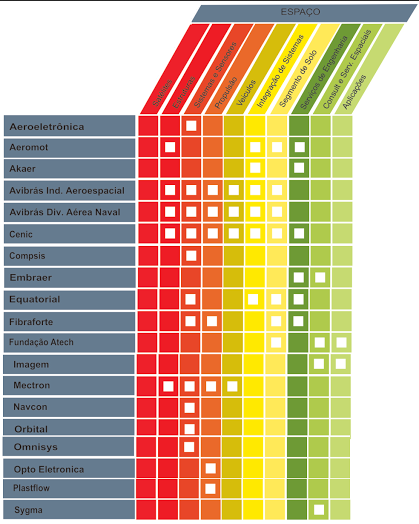
\includegraphics[width=0.8\linewidth]{./figs/Figura_08}
			
		\begin{small}
			FONTE: Adaptado da Associação das Indústrias Aeroespaciais do Brasil
		\end{small}		
	\end{figure}
		
	As empresas focam nos sistemas secundários e de menor complexidade, como visto na Figura \ref{Segmentação}, optando no desenvolvimento, principalmente, de sensores e segmento de solo.
		
\section[Clientes]{Clientes}

	O público alvo da CuboBrasil será as Instituições de Ensino e/ou Pesquisa, centros militares e pessoas que utilizam o CubeSat como uma forma de \textit{hobby} que se localizem no Brasil.
	
	Os clientes são pessoas que gostam e tem acesso à alta tecnologia mundial, com interesses acadêmicos, militares ou simplesmente visando lucro, que se encontram especificamente nos grandes centros tecnológicos do mundo.


\subsection[Concorrência]{Concorrência}

	No Brasil essa tecnologia é recente e escassa, sendo assim uma área a ser desenvolvida e consolidada nacionalmente, isto pelo fato de possuir custo elevado e requerer tempo dedicado à pesquisa de novas tecnologias.
	
	A empresa vem com o \textit{know-how}, plataforma e condições necessárias para sanar a carência que o mercado nacional possui no setor aeroespacial, oferecendo tecnologia de ponta, novos conceitos e facilidades de acesso a seus produtos.
	
	Fazendo uma análise dos dados da Tabela 1, é possível notar a superioridade de qualidade da GomSpace, porém pela empresa não adotar políticas de facilidades no pagamento e por estar localizada no exterior, o que implica em fretes mais elevados e taxas de importação, a CuboBrasil encontra uma oportunidade para entrar no mercado e começar a galgar seu espaço no cenário nacional. Se consolidando no mercado brasileiro as portas da América Latina se abrem com maior facilidade, uma vez uma empresa localizada nessa região barateia os custos de transportes e taxas (aproveitando alguns acordos econômicos, como o Mercosul). 
	
	Com relação a CubeSatKit, a CuboBrasil explorará a qualidade do produto, além da localização, para ganhar um pedaço do mercado, uma vez que os clientes tendem a não levar somente o preço em consideração na hora de realizar as compras dos produtos com alto tecnologia associada.
	
	A disputa contra a CubeSatShop será baseada no preço, uma vez que a qualidade dos produtos de ambas são similares o fator preço pode beneficiar a CuboBrasil numa possível comparação realizada pelos clientes. Novamente a localização das empresas podem pesar a favor de uma ou outra na hora da aquisição dos produtos.
	
	\begin{table} [th]
	\label{tab_comp_forn}
	\caption{COMPARATIVO ENTRE CUBOBRASIL E CONCORRÊNTES}
	\centering
	\begin{tabular}{|p{3cm}|p{2.5cm}|p{2.5cm}|p{2.5cm}|p{2.7cm}|}
	\hline
	\textbf{Empresa} & CuboBrasil & GomSpace & CubeSatkit & CubeSatShop \\
	\hline
	\textbf{Qualidade} & Boa & Ótima & Razoável & Boa \\
	\hline
	\textbf{Preço} & Bom & Alto & Baixo & Alto\\
	\hline
	\textbf{Condições de\linebreak Pagamento} & Sem\linebreak facilidades & Sem\linebreak facilidades & Facilitado & Facilitado\\
	\hline
	\textbf{Localização} & São Paulo\linebreak Brasil & Aalborg\linebreak Dinamarca & São Francisco\linebreak EUA & Delft\linebreak Holanda\\
	\hline
	\textbf{Atendimento} & Internet\linebreak Telefone & Internet\linebreak Telefone & Internet\linebreak Telefone & Internet\linebreak Telefone \\
	\hline
	\textbf{Serviços\linebreak adicionais} & Treinamento\linebreak Cursos\linebreak Manutenção\linebreak Assistência técnica & Não possui & Não possui & Não possui\\
	\hline
	\textbf{Garantia} & Sim & Sim & Sim & Sim\\
	\hline
	
	\end{tabular}
	
	\begin{small}
		FONTE: Elaborada pelos autores através de pesquisas realizadas nos sites das empresas.
	\end{small}
	\end{table}	
	\pagebreak
	
	Entendendo os critérios adotados na Tabela 1 pode-se ter uma ideia de como são os planos de negócios delas. 
	
	O item \textbf{Qualidade} têm os seguintes critérios de avaliação: ruim, razoável, boa e ótima. Essa característica leva em conta os componentes utilizados e o procedimento de montagem dos produtos.
	
	\begin{itemize}
		\item Ruim
		 
		Componentes sem nenhuma especificação requerida e procedimento de montagem totalmente fora dos padrões necessários para o projeto.
		
		\item Razoável
		
		Componentes selecionadas com baixo critério, muitas vezes adaptados a disponibilidade e/ou custo, existe procedimento de montagem porém não atendido 100\%.
		
		\item Boa
		
		Uso de componentes de primeira linha e procedimento de montagem realizado corretamente.
		
		\item Ótima
		
		Uso de componentes específicos (linha de produtos destinada ao segmento aeroespacial) e procedimento de montagem realizado corretamente em salas limpas.		
		
	\end{itemize}

	 Já o item \textbf{Preço} possui os seguintes critérios de avaliação: baixo, bom e alto. Esse item foi avaliado relacionando o custo de um produto de qualidade boa com a qualidade apresentada no produto.
	 
	 \begin{itemize}
	 
	 	\item Baixo
	 	
	 	Preço mais baixo do mercado para um produto com uma qualidade inferior. Produto com baixo lucro para o fabricante e de baixo custo-benefício para o comprador.
	 	
	 	\item Bom
	 	
	 	Preço competitivo de mercado, possui um bom lucro para o fabricante e um bom custo-benefício para o cliente.
	 	
	 	\item Alto
	 	
	 	Preço elevado, com uma excelente lucro para o fabricante e um bom custo-benefício para o usuário.
	 	
	 \end{itemize}
	
	Tendo claro os critérios utilizados no comparativo anterior, pode-se agora ter uma ideia do plano de negócios dos concorrentes existentes.
	
	\subsubsection[GomSpace]{GomSpace}
	
	A dinamarquesa \textit{\textbf{GomSpace}}, trabalha somente com produtos de alta qualidade, porém possui o maior preço do mercado. Esse preço elevado restringe um pouco do seu \textit{market share} uma vez que o público hobista não está disposto a gastar grandes quantias, além de não tem capacidade financeira de financiar o lançamento do seu \textit{CubeSat}.
	
	\textbf{Mercados de interesse:} instituições de ensino, área militar e centros de pesquisas.
	
	\begin{minipage}{7cm}
	\begin{center}
	\textbf{Vantagens}
	\end{center}
	
	\begin{itemize}
	\item \textit{Know-how} elevado
	\item Alta qualidade e confiabilidade
	\item \textit{Lead time}
	\end{itemize}
	\end{minipage}
	\begin{minipage}{7cm}
	\begin{center}
	\textbf{Desvantagens}
	\end{center}
	
	\begin{itemize}
	\item Sem serviços adicionais
	\item Alto custo de investimento
	\item Baixa flexibilidade do produto
	\end{itemize}		
	\end{minipage}
	
	\subsubsection[CubeSatKit]{CubeSatKit}
	
	A americana \textit{\textbf{CubeSatKit}}, visa o ganho de \textit{market share} através do público hobbista, uma vez que possui o produto mais barato do mercado, com facilidade de pagamento, atendendo a expectativa desse público, que até então não estava no foco dessas empresas. Possui um baixo custo de operação, pois não faz questão de utilizar todos os componentes com alto padrão de qualidade. Porém essa qualidade inferior impacta diretamente na qualidade do produto.
	
	\textbf{Mercados de interesse:} hobistas, instituições de ensino e centros de pesquisas.
	
	\begin{minipage}{7cm}
	\begin{center}
	\textbf{Vantagens}
	\end{center}
	
	\begin{itemize}
	\item Baixo custo
	\item Pagamento facilitado
	\item Fidelização do cliente
	\end{itemize}
	\end{minipage}
	\begin{minipage}{7cm}
	\begin{center}
	\textbf{Desvantagens}
	\end{center}
	
	\begin{itemize}
	\item Sem serviços adicionais
	\item Baixa flexibilidade do produto
	\item Qualidade e confiabilidade questionáveis
	\end{itemize}		
	\end{minipage}
	
\subsubsection[CubeSatShop]{CubeSatShop}
	
	A holandesa \textit{\textbf{CubeSatShop}}, possui produtos com boa qualidade e um preço competitivo. Com foco na venda dos subsistemas dos \textit{CubeSats} desenvolvidos por eles. Devido a relação preço e qualidade, além da facilidade de pagamento, briga para aumentar seu \textit{market share} em todos os segmentos do mercado.
	
	\textbf{Mercados de interesse:} hobistas, área militar, instituições de ensino e centros de pesquisas.
	
	\begin{minipage}{7cm}
	\begin{center}
	\textbf{Vantagens}
	\end{center}
	
	\begin{itemize}
	\item Pagamento facilitado
	\item Preço competitivo
	\item Boa qualidade e confiabilidade
	\end{itemize}
	\end{minipage}
	\begin{minipage}{7cm}
	\begin{center}
	\textbf{Desvantagens}
	\end{center}
	
	\begin{itemize}
	\item Sem serviços adicionais
	\item Baixa flexibilidade do produto
	\item Logística
	\end{itemize}		
	\end{minipage}
	
\subsection[Fornecedores e prestadores de serviço]{Fornecedores e prestadores de serviço}

	Para o desenvolvimento dos módulos e dos produtos, nossa sensibilidade aos fornecedores é extremamente forte, acreditamos que seja da ordem de 90\%. Isso, pois todos os componentes para a fabricação das placas são importados e há pouco ou quase nenhum fornecedor alternativo.
	
	\begin{table} [th]
	\caption{INFORMAÇÕES DOS PRINCÍPAIS FORNECEDORES}
	\centering
	\begin{tabular}{|p{2.3cm}|p{2.5cm}|p{2.5cm}|p{1.6cm}|p{1.4cm}|p{1.7cm}|}
	\hline
	\textbf{Fornecedor} & Farnell & Digikey & Grifos & TrisolX & AzurSpace \\
	\hline
	\textbf{Item} & Componentes & Componentes & PCB & Células Solares & Células Solares\\
	\hline
	\textbf{Preço} & Alto & Bom & Baixo & Baixo & Alto\\
	\hline
	\textbf{Condição\linebreak Pagamento} & À vista & À vista & Facilitado & À vista & À vista \\
	\hline
	\textbf{Prazo} & 4 semanas & 4 semanas & 5 dias & 2 semanas & 10 semanas\\
	\hline
	\textbf{Localização} & Reino Unido & EUA & Brasil & EUA & Alemanha \\
	\hline
	
	\end{tabular}
	
	\begin{small}
		FONTE: Elaborada pelos autores através de pesquisas realizadas nos sites das empresas.
	\end{small}
	\end{table}
	
\section[Posicionamento]{Posicionamento}	

	O posicionamento estratégico da empresa no mercado é de extrema importância, pois é ele que irá irá ajudar a empresa a atingir todos os seus objetivos de pequeno, médio e longo prazo.

\subsection[Segmentação do mercado]{Segmentação do mercado}

	O público alvo da CuboBrasil são universidades, institutos de pesquisa e desenvolvimento, defesa militar e hobistas.
	
	Visando as necessidades especificas de cada cliente, a CuboBrasil espera suprir as principais demandas de cada grupo. Sabendo-se que, um determinado produto não atende as especificações de todos os grupos de clientes, será necessário adaptações no projeto para poder abranger todos os segmentos.
	
	Universidades, institutos de pesquisa e desenvolvimento, visam o estudo da tecnologia para diversos fins, como por exemplo para fomentar a pesquisa e desenvolvimento de projetos para formar e capacitar alunos e pesquisadores na área espacial ou realizar determinados experimentos nas condições oferecidas pelo espaço.
	
	Já a área militar, pode se beneficiar da utilização do produto de diversas formas, como por exemplo o monitoramento de possíveis desmatamentos, identificação de aeroportos clandestinos, plantações de drogas, acompanhamento de operações militares entre outras.
	
	O público hobista possui diversas peculiaridades. Entende-se por \textit{hobby} uma atividade que é praticada por prazer durante os tempos livres, porém existem uma infinidade de diferenças entre os próprios hobistas e o seu grau de interesse pelo \textit{hobby} que pratica. Esse grau de interesse tem um grande impacto nessa fatia do mercado, pois existem tanto aqueles que são altamente engajados e possuem um vasto conhecimento sobre o sistema e de que forma poderia utizá-lo como também têm aqueles que estão despertando o interesse pelo assunto aeroespacial agora e possuem baixo nível de conhecimento do mesmo. Esse público, na sua grande maioria, dificilmente tem condições de financiar o lançamento do produto para o espaço e acabam utilizando-o mais como uma ferramenta para estudo de rádio amadorismo, entre outros.
	
	De forma geral, entende-se que:
	
	\begin{table} [th]
	\caption{CLIENTES E PRINCIPAIS CARACTERÍSTICAS}
	\centering
	\begin{tabular}{p{6cm}|p{6cm}}

		\textbf{Cliente} & \textbf{Características}\\
		\hline
		Universidades, Institutos de pesquisa e desenvolvimento & Verba moderada, conhecimento superficial do funcionamento do sistema, adaptável ao produto disponível\\
		\hline
		Área militar & Verba alta, conhecimento sólido do funcionamento do sistema, busca confiabilidade e segurança do produto, exigência de produto customizado\\
		\hline
		Hobistas & Verba escassa, variados níveis de conhecimento do funcionamento do sistema, adaptável ao produto disponível\\
		\hline
			
	\end{tabular}
	
	\begin{small}
		FONTE: Elaborada pelos autores através de pesquisas realizadas nos sites das concorrentes.
	\end{small}	
	\end{table}		
	\pagebreak
	A empresa deseja, inicialmente, um \textit{market share} de 2\% do mercado de \textit{CubeSats} no mundo.
	 
 	Estima-se que sejam vendidos cerca de 100 \textit{CubeSats}, a Figura 4 representa a estimativa percentual dos concorrentes da CuboBrasil representam no mercado atual. 
 	
 	\begin{figure}[th]
		\caption{ESTIMATIVA PERCENTUAL DO MERCADO DE CUBESATS}
		\centering
		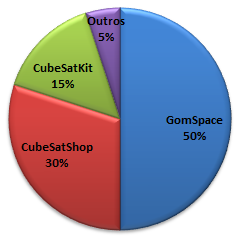
\includegraphics[width=0.5\linewidth]{./figs/Figura_04}
		
		\begin{small}
			FONTE: Elaborado pelos autores, através de levantamento realizado nos sites de projetos correntes e das empresas do segmento.
		\end{small}
	\end{figure}
 	\pagebreak
 	Diante do acordo firmado, em Julho de 2014, entre a Agência Brasileira de Promoção de Exportações e Investimentos (Apex-Brasil) e o Centro para a Competitividade e Inovação do Cone Leste Paulista (Cecompi) que visa promover negócios e a imagem de produtos e serviços da indústria aeroespacial, eles esperam que um crescimento de mais de 30\% no volume exportado de produtos e serviços. Baseado nesse acordo, a CuboBrasil tem uma expectativa otimista de ter um crescimento de 50\% no volume de vendas.
	
\subsection[Posicionamento estratégico]{Posicionamento estratégico}

	O posicionamento estratégico de uma empresa está voltado para o atendimento com os públicos de interesse, cada público deve ser tratado de forma única, por tanto as ações que a empresa irá tomar depende do comportamento desses públicos. Como o foco da CuboBrasil está em Universidades, Institutos de pesquisa e desenvolvimento, Militar e hobistas, foi levantado o perfil de cada tipo de cliente.

	\begin{itemize}
		\item Universidades, Institutos de pesquisa e desenvolvimento:
		
		O produto por ser nacional possui facilidade de aquisição e a possibilidade de aumento de conhecimento com treinamentos e consultoria que estão disponíveis em um plano de negócio, que diferentemente dos concorrentes que estão fora e só oferecem produtos prontos e não esses tipos de serviço.
		
		\item Militar:
		
		Vantagem de personalização do produto, o produto pode se adequar de acordo com necessidades, devido a possuirmos tecnologia e \textit{know-how} referente ao produto, para podermos atender especificações que os concorrentes não atenderiam normalmente já que trabalham apenas com módulos prontos.
		
		\item Hobistas:
		
		Baixo custo e um curto prazo de entrega em relação aos principais concorrentes.
	\end{itemize}
	
\section[Estratégias de marketing]{Estratégias de marketing}

	Os produtos oferecidos pela CuboBrasil são: placa de gerenciamento de energia, placa de comunicação, placa mãe e o \textit{CubeSat} completo.
	
	Esse portfólio tem o diferencial da tecnologia nacional a um preço mais acessível, curto prazo de entrega e a facilidade do cliente entrar em contato com a assistência técnica.
	
\subsection[Preço]{Preço}

	 A precificação dos produtos foi baseada no custo para a montagem dos módulos mais lucro, levando em conta o quanto o cliente estaria disposto a pagar pelos produtos dos principais concorrentes, como é demonstrado nas Figuras 5, 6 e 7.
	 
	 \begin{figure}[th]
		\caption{COMPARAÇÃO DE PREÇO ENTRE CUBOBRASIL E CONCORRENTES}
		\centering
		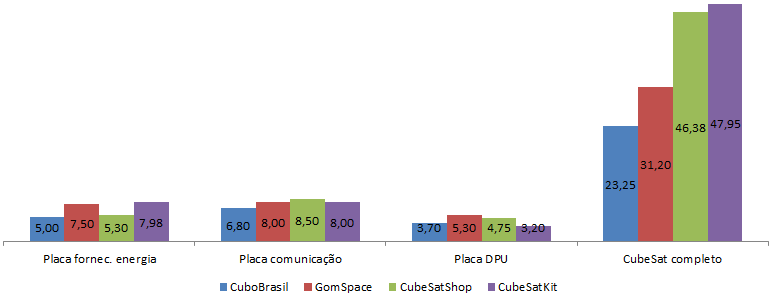
\includegraphics[width=1.0\linewidth]{./figs/Grafico_01}
		
		\begin{small}
			FONTE: Elaborado pelos autores, através de levantamento realizado no site das empresas.
		\end{small}
		
		\begin{footnotesize}
			NOTA: Valores em milhares de Euros.
		\end{footnotesize}
	\end{figure}

	\begin{figure}[th]
		\caption{DEMONSTRATIVO DE GASTOS PARA CADA PRODUTO VENDIDO}
		\centering
		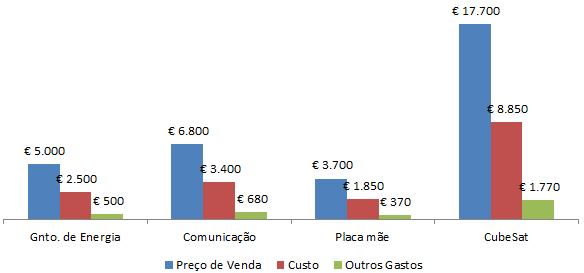
\includegraphics[width=1.0\linewidth]{./figs/Figura_05}
		
		\begin{small}
			FONTE: Elaborado pelos autores, através de levantamento realizado de componentes e serviços necessários.
		\end{small}
	\end{figure}
	\pagebreak	
	\begin{figure}[ht]
		\caption{DEMONSTRATIVO DA PREVISÃO DE FATURAMENTO E LUCRO DA CUBOBRASIL}
		\centering
		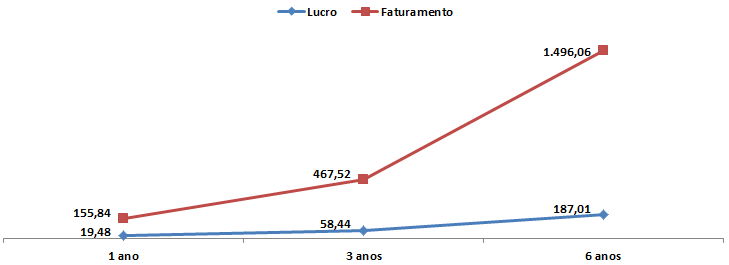
\includegraphics[width=1.0\linewidth]{./figs/Grafico_02}
		
		\begin{small}
			FONTE: Elaborado pelos autores, através de análise do mercado.
		\end{small}
		
		\begin{footnotesize}
			NOTA: Valores em milhares de Euros.
		\end{footnotesize}
	\end{figure}	
	
\subsection[Praça]{Praça}	

	Vendas serão realizadas por meio de site (\textit{on-line}) e representantes com disponibilidade de visita ao cliente.
	
\subsection[Promoção]{Promoção}
	
	Hoje em dia a comunicação é a melhor maneira de interagir com o público, para ganhar destaque na mente do consumidor, uma boa divulgação de seu negócio é essencial.
	
  	Dados mostram que para ganhar um \textit{marketing share}, uma boa propaganda é a solução, ela tem a função de expor da melhor forma possível o que o produto vai oferecer aos seus consumidores, tem também a função de tornar a empresa conhecida no mercado.
  	
	A publicidade de nossa empresa está direcionada para os clientes alvo de cada segmento de mercado, e são:
	
	\begin{itemize}
		\item Propagandas em revistas de tecnologia, aeroespaciais e as de maiores destaques entre o público intelectual;
		\item Propagandas na internet, servindo de base, este tipo de anuncio será feito através de links, que direcionam a curiosidade das pessoas para o site da empresa, em redes sociais, onde pessoas já possuem comunidades ou grupos online que tratam de assuntos específicos desta área, onde a vitrine para os produtos torna-se algo muito interessante;
		\item \textit{Outdoor}, de acordo com especialistas na área de publicidade e propaganda, este é um dos meios, junto a televisão e rádio, com maior eficácia, pois tem um alto impacto visual, oferecendo altos índices de \textit{recall} (lembrança), demonstrando um aproveitamento de mais de 70\% de retorno. Neste caso as propagandas da empresa trabalharam a imagem da marca, despertando curiosidade, propagandas colocadas em lugares estratégicos, próximos aos locais onde estão os possíveis clientes, criando uma relação entre clientes e empresa, pois o anuncio é visto com grande frequência pelo público alvo, que transita várias vezes pelo local;
		\item Participação em feiras e eventos, neste caso o público alvo vai ao local com interesses já formados, por se tratar de um público altamente dirigido e qualificado. Nestes eventos serão oferecidos brindes e existirão sorteios de produtos, que façam com que os clientes não esqueçam da CuboBrasil, mostrando um pouco da história, produtos e novas tecnologias. Esse público também poderá contar cursos e treinamentos direcionados.	
	\end{itemize}

\subsection[Relacionamento com os clientes]{Relacionamento com os clientes}
	
	O relacionamento com o cliente será baseado na segmentação dos mesmos contando com formatos que se adequam a todos.
	 
	A estratégia que será adotada de forma que se crie um relacionamento com todos é a vinculação de \textit{newsletters} (boletins informativos) mensais que irão dispor de conteúdos referentes às novidades aeroespaciais, artigos e divulgação de novas funcionalidades e equipamentos disponíveis pela CuboBrasil.

	Tratando-se de universidades, institutos de pesquisa e desenvolvimento, serão disponibilizados treinamentos e \textit{workshops} com o intuito de aumentar o conhecimento sobre o funcionamento do sistema.
	
	O relacionamento com a área militar também conterá treinamentos e \textit{workshops}, porém, por se tratar de um segmento de mercado que possui um bom conhecimento do funcionamento do sistema, serão disponibilizados cursos com uma complexidade elevada na qual irão ser abordados temas como a customização dos sistemas para uma obtenção mais rica em detalhamento das missões realizadas.
	
	Como os hobistas representam uma pequena parcela do mercado e que devido ao custo dos equipamentos não possibilitarem uma alta frequência de aquisição dos kits, o relacionamento com eles será realizado basicamente com as \textit{newsletters} e com alguns cursos mais elementares.

\section[Forças de Porter]{Forças de Porter}

	O modelo das cinco forças de Porter	permite avaliar de forma mais profunda a competição entre as empresas permitindo um desenvolvimento de modelo estratégico mais acurado. Essas forças atuam como ameaça no desempenho da indústria e, por consequência, nas empresas podendo ou não comprometer o desempenho empresarial.

	\begin{figure}[th]
		\caption{FORÇAS DE PORTER}
		\centering
		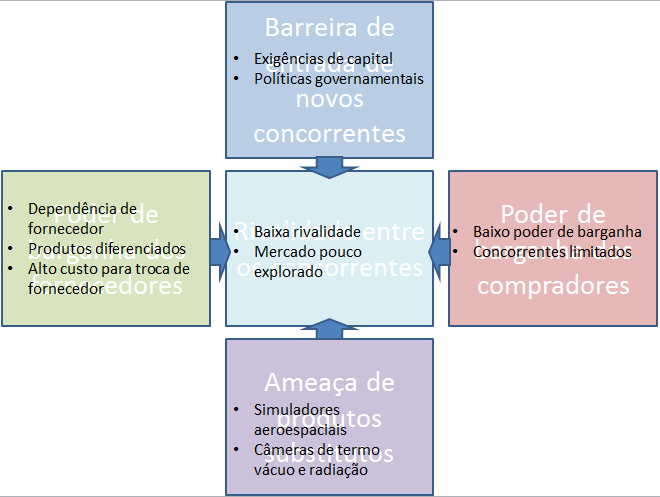
\includegraphics[width=1.0\linewidth]{./figs/PORTER}
		
		\begin{small}
			FONTE: Elaborado pelos autores.
		\end{small}
	\end{figure}

\section[Análise SWOT]{Análise SWOT}

	A análise SWOT é de fundamental importância para o planejamento de um negócio. De forma resumida, é uma ferramenta estrutural da administração, que visa avaliar os ambientes internos e externos para a formulação de estratégias de negócio para a otimização do desempenho no mercado.
	
	\begin{figure}[th]
		\caption{SWOT DA CUBOBRASIL}
		\centering
		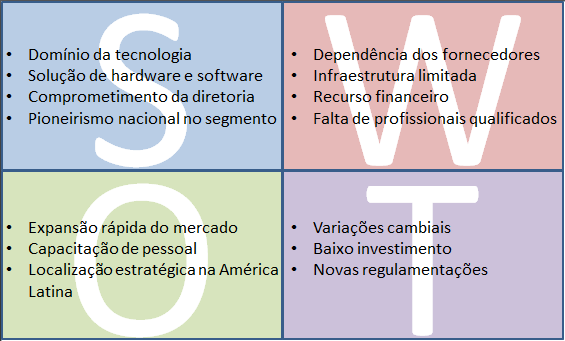
\includegraphics[width=1.0\linewidth]{./figs/SWOT}
		
		\begin{small}
			FONTE: Elaborado pelos autores.
		\end{small}
	\end{figure}	
	\pagebreak
\subsection[Strenghts]{\textit{Strenghts}}

	O domínio da tecnologia advém da formação técnica e do estudo sobre esse mercado que se iniciou no período de graduação dos empreendedores. O que os tornou capazes de desenvolver sua própria solução otimizada de \textit{hardware} e \textit{software}.
	
	O pioneirismo nacional está totalmente relacionado com o comprometimento da diretoria que, além de trabalhar de forma árdua no crescimento da empresa, realizou diversas pesquisas de mercado para identificar o melhor polo aeroespacial dentro da América Latina.

\subsection[Weaknesses]{\textit{Weaknesses}}

	Devido ao baixo investimento governamental em tecnologia nacional e de qualificação de pessoas para o desenvolvimento de alta tecnologia, a alternativa encontrada é a importação desses elementos e componentes, o que acaba elevando os custos e tornando a empresa extremamente dependentes dos fornecedores, os quais ainda são limitados. 
	
	A infraestrutura é limitada, não só pela baixa verba, mas também pela necessidade de importação dos equipamentos necessários para o desenvolvimento dos produtos.

\subsection[Opportunities]{\textit{Opportunities}}

	Mesmo com o baixo investimento nacional, os \textit{CubeSats} criaram uma nova esfera do mercado para o desenvolvimento de tecnologias aeroespaciais, o que possibilita, para quem detém o conhecimento dessa tecnologia, uma rápida expansão no mercado. 
	
	A CuboBrasil está estrategicamente localizada no maior polo aeroespacial da América Latina, que é o estado de São Paulo, se aproveitando dessa oportunidade para a gerar a captação técnica e mão de obra especializada necessária.

\subsection[Threats]{\textit{Threats}}
	
	Embora o mercado esteja crescendo e se destacando de forma global, ocorre que no Brasil ainda existe pouco interesse de investidores, por ainda não existir regulamentações técnicas que estabeleçam as regras para o setor aeroespacial brasileiro.
	
	Ainda existe, também, os fatores relacionados as variações cambiais, o que deixa a empresa extremamente suscetível ao aumento do dólar nas transações comerciais.
	
\chapter[Plano Operacional]{Plano Operacional}

	O Plano Operacional visa operacionalizar a empresa, ou seja, explicar ao empresário todas as questões referentes ao ambiente físico desta.
 
	Serão levantados todos os materiais necessários bem como serão definidos os fornecedores em conjunto com o cliente. De acordo com cada empresa serão definidos quantos funcionários serão necessários e qual sua remuneração.
 
	Além disso todos os documentos necessários para o empreendimento serão elencados para que os clientes tenham todas as diretrizes para abrir ou manter seu negócio com segurança. O Plano Operacional também dá insumos para a realização do Plano Financeiro.

\section[Produtos e serviços]{Produtos e serviços}

	A CuboBrasil, possui os seguintes produtos e serviços:
	

	\textbf{Produtos}
	
	\begin{itemize}
		\item \textit{CubeSat} completo;
		\item \textit{Energy Power System};
		\item \textit{Communication System};
		\item \textit{Data Processing Unit};
		\item \textit{Control System}.
	\end{itemize}

	\textbf{Serviços}
	
	\begin{itemize}
		\item Treinamento;
		\item Suporte técnico;
		\item Serviços de rádio base.
	\end{itemize}


	Na sequência será apresentado de forma detalhada o \textit{Energy Power System} ou simplesmente \textit{EPS}. Na Figura \ref{produtos} é apresentado o \textit{kit} de um \textit{EPS} completo disponibilizado pela CuboBrasil.
	
		\begin{figure}[th]
		\caption{\textit{EPS} OFERECIDO PELA CUBOBRASIL}
		\label{produtos}
		\centering
		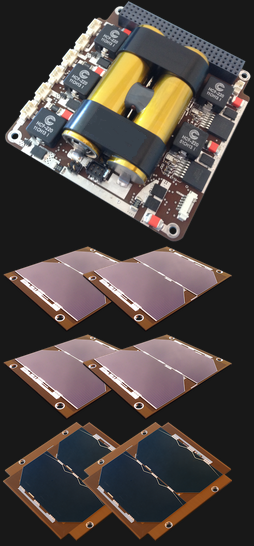
\includegraphics[width=0.3\linewidth]{./figs/produtos}
		
		\begin{small}
			FONTE: GOMSpace.
		\end{small}
	\end{figure}\pagebreak
	
	\begin{itemize}
		\item[\textbf{EPS}]
		O \textit{EPS} da CuboBrasil, fornece uma solução de potência total para qualquer missão de \textit{CubeSat}, incluindo funções como rastreamento da máxima potência, gestão de carregamento e distribuição de energia e um \textit{pack} de baterias, tudo em uma única placa. O \textit{kit} completo é composto por 1 \textit{power module} e 6 placas de fotocélulas, sendo que cada uma dessas placas possuem um sensor solar. Produto totalmente compatível com qualquer outro oferecido pela CuboBrasil.
	\end{itemize}
	
	A configuração básica do produto para um \textit{CubeSat} de uma unidade, é representada na Figura \ref{configuracao}.
	
	\begin{figure}[th]
		\caption{CONFIGURAÇÃO DO \textit{EPS}}
		\label{configuracao}
		\centering
		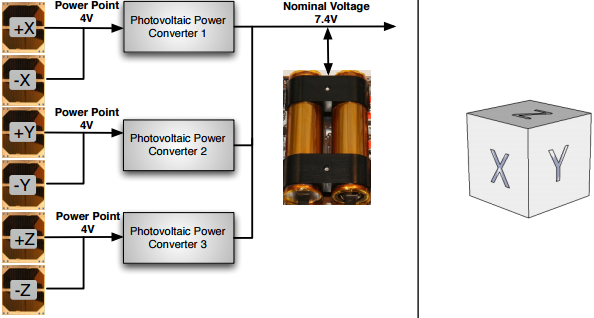
\includegraphics[width=0.55\linewidth]{./figs/configuracao}
		
		\begin{small}
			FONTE: GOMSpace.
		\end{small}
	\end{figure}
	
	As especificações técnicas do produto são:
	
	\textbf{Especificações elétricas:}
	
	\begin{itemize}
		\item Alimentação fotovoltaíca para até 30W;
		\item Três barramentos de alimentação reguladas: 3,3V, 5V e 12V;
		\item Saídas: 3,3V@3A, 5V@2A e 12V@1A;
		\item Capacidade da bateria: 2700 mAh.
	\end{itemize}
	
	\textbf{Propriedades físicas:}
	
	\begin{itemize}
		\item Temperatura operacional: Intervalo industrial;
		\item Material da PCB: Vidro/Poliimida IPC6012C cl. 3/A;
		\item IPC-A-610 Classe 3 montagem.
	\end{itemize}
	
\section[Unidade operacional]{Unidade operacional}
	
	Devido à ausência de dependência entre nossos futuros clientes e dos nossos fornecedores ao local escolhido para a sede da CuboBrasil, uma vez que os cursos poderão ser realizados no próprio cliente e os produtos, assim como as matérias primas, serão entregues pela equipe de transporte, decidiu-se avaliar as locações na região do ABC Paulista (Santo André, São Bernardo do Campo e São Caetano do Sul), pois, além do fácil acesso, o ABC Paulista é próximo da cidade em que serão realizados as análises dos produtos vendidos pela empresa e das moradias da maioria dos sócios.
	
	Foi realizada uma pesquisa de preço de locação de salas e casas comerciais, na qual resultou que São Caetano do Sul é a cidade mais barata entre as três, seguida de Santo André e São Bernardo do Campo. O valor encontrado por metro quadrado é de R\$ 22.65, R\$ 34.69 e R\$ 41.17, respectivamente. Por se tratarem de salas comerciais todos os locais pesquisados atendem a legislação, para as atividades necessárias da CuboBrasil necessita-se encontrar um local que tenha uma sala para reuniões e realização dos treinamentos, uma sala para a equipe técnica, outra para o administrativo, recepção, banheiro e uma copa.
	
	O local escolhido para sediar a CuboBrasil foi uma sala comercial no bairro de Nova Gerti em São Caetano do Sul, São Paulo, cujo aluguel é no valor de R\$ 1200,00 e o tamanho é de 80 m\textsuperscript{2}, o qual atende plenamente todas as necessidades da CuboBrasil. 
	
\section[Tecnologia e processos]{Tecnologia e processos}

	Os processos e tecnologias utilizados para atender as necessidades da CuboBrasil são fundamentais para capturar e armazenar o conhecimento organizacional da empresa. A tecnologia Tecnologia aplicada na produção é nacional adaptada a cada necessidade de projeto. Por se tratar de projetos customizados, a automatização do processo produtivo não pode ser viabilizada, dessa forma boa parte dos produtos oferecidos são desenvolvidos manualmente.

\section[Descrição dos processos e operações]{Descrição dos processos e operações}

	Nas Figuras \ref{X} e \ref{X-1}, é exibido o fluxograma geral do processo em relação a solicitação de produtos e serviços.
	
	\begin{figure}[th]
		\caption{FLUXOGRAMA GERAL DO PROCESSO EM RELAÇÃO AOS PRODUTOS}
		\label{X}
		\centering
		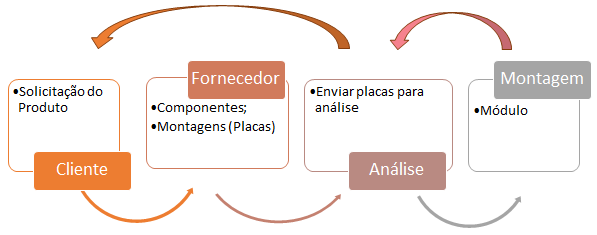
\includegraphics[width=1.0\linewidth]{./figs/X}
		
		\begin{small}
			FONTE: Elaborado pelos autores.
		\end{small}
	\end{figure}
	
	O processo em relação aos produtos começa com a “Solicitação do Cliente”, logo após a verificação dos componentes necessários para a montagem do produto é feita uma solicitação aos fornecedores.
	
	Ao receber os materiais é realizada a montagem das placas, que são enviadas para um parceiro onde podem ser feitos testes que comprovem seu funcionamento. Uma vez que, as placas estejam de acordo, as mesmas retornam a sede da empresa juntamente com um laudo de conformidade, que posteriormente será enviado para o cliente.
	
	Já para a solicitação de serviço existem três etapas: A solicitação do cliente, assim como para o produto, a análise da solicitação na qual é feita uma cotação do serviço discriminando o local, data e conteúdo, caso sejam cursos, e pôr fim a execução do mesmo.
	 
	 \begin{figure}[th]
		\caption{FLUXOGRAMA GERAL DO PROCESSO EM RELAÇÃO AOS SERVIÇOS}
		\label{X-1}
		\centering
		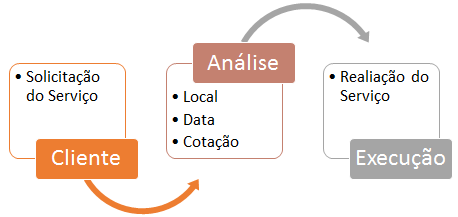
\includegraphics[width=0.8\linewidth]{./figs/X-1}
		
		\begin{small}
			FONTE: Elaborado pelos autores.
		\end{small}
	\end{figure}
	
	

\section[Arranjo físico e recursos produtivos]{Arranjo físico e recursos produtivos}

	O \textit{layout} do escritório da CuboBrasil foi desenvolvido pensando na necessidade da empresa. A divisão de salas foi realizada da seguinte forma: setor administrativo, setor de engenharia e área comum, que é constituída por uma sala de reunião, onde além de reuniões serão ministrados os cursos e treinamentos, uma copa que poderá ser utilizada tanto por funcionários quanto por clientes, fornecedores e parceiros, um banheiro e uma recepção. Esta divisão será detalhada a seguir e poderá ser observada na Figura \ref{layout}.
	
	\begin{figure}[th]
		\caption{\textit{LAYOUT} DA CUBOBRASIL}
		\label{layout}
		\centering
		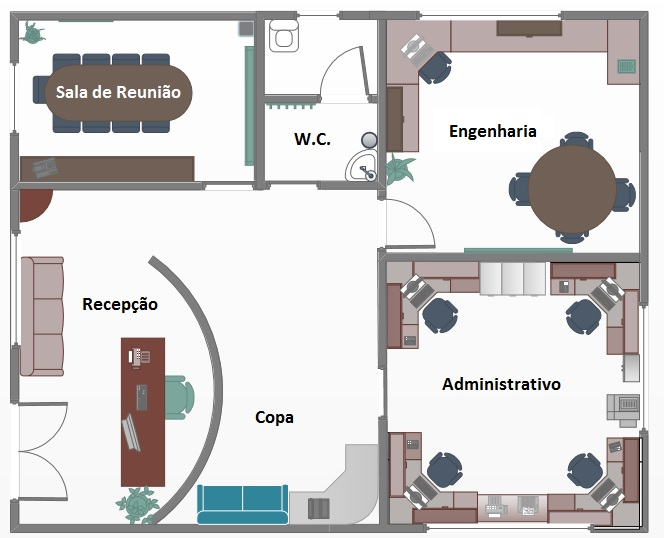
\includegraphics[width=0.7\linewidth]{./figs/layout}
		
		\begin{small}
			FONTE: Elaborado pelos autores.
		\end{small}
	\end{figure}\pagebreak
	
 	No setor administrativo, encontram-se as pessoas responsáveis pera área comercial, financeira, marketing e de logística, assim a comunicação entre as áreas será mais rápida e eficiente. Os equipamentos necessários a este setor são: telefone, fax, copiadora/scanner, picotadeira de papel e quatro computadores. Os móveis selecionados para este setor são: quatro mesas de canto com um gaveteiro cada, quatro armários suspenso, três arquivos, um gaveteiro comum e quatro cadeiras.
 	
	No setor de engenharia, encontram-se as pessoas responsáveis pelos produtos e serviços oferecidos pela CuboBrasil. Os ítens deste setor são: uma mesa de canto com gaveteiro, um computador, um telefone, uma bancada para montagem, embalagem e armazenamento do produto até que ele seja enviado para o laboratório ou cliente, dois armários suspensos, uma mesa redonda e cinco cadeiras e um quadro branco, além de equipamentos básicos de desenvolvimento, como ferro de solda, fonte, osciloscópio, geradores de frequência, entre outros.
	
	A sala de reunião é composta por uma mesa grande e nove cadeiras, um armário-bancada, um projetor e um painel de projeção.
	
	A copa foi projetada pensando no \textit{coffee break} tanto dos funcionários quanto dos clientes que estejam visitando o escritório para alguma reunião ou curso/treinamento. Nela se encontra um sofá de dois lugares, uma bancada em “L”, uma cafeteira nespresso e aperitivos como pães, bolachas, biscoitos, bolos etc.
	
	Dizem que a primeira impressão é a que fica, por isto a recepção foi projetada visando o conforto do cliente, para que ele se sinta “em casa” podendo ser um diferencial a mais. Pois além da qualidade a CuboBrasil preza pelo bom tratamento de seus clientes. Os ítens da recepção são: um sofá de três lugares, uma mesa com revistas sobre tecnologia e ítens relacionados aos produtos oferecidos, uma mesa, um telefone/fax, um computador e um painel com a marca da empresa.
	
\subsection[Descrição dos cargos]{Descrição dos cargos}

	Para a realização das funções de cada área serão necessários funcionários capacitados. A seguir serão apresentadas as descrições de cargos necessárias para as contratações dos funcionários da CuboBrasil.
	
	\begin{itemize}
		\item Auxiliar administrativo
		\subitem Hierarquia: Financeiro/Administrativo;
		\subitem Formação necessária: Ensino superior (Engenharia, Administração e Contabilidade);
		\subitem Requisitos da função: Inglês intermediário;
		\subitem Carga horária: 40 horas semanais;
		\subitem Tipo de contratação: CLT;
		\subitem Faixa salarial: 816,00 - 1371,00 - 2075,00;
		\subitem Experiência: 6 meses;
		\subitem Descritivo das atividades: Executar serviços administrativos, abertura de ordem de serviços, fechamento e rateio das faturas mensais, controle de documentação, acompanhamento de auditoria interna e externa, controle e elaboração de planilhas e relatórios, confeccionar cronograma, fluxograma e organograma.
		
		\item Vendedor
		\subitem Hierarquia: Comercial;
		\subitem Formação necessária: Ensino superior (Engenharia);
		\subitem Requisitos da função: Inglês intermediário;
		\subitem Carga horária: 40 horas semanais;
		\subitem Tipo de contratação: CLT;
		\subitem Faixa salarial: 1752,00 - 2087,00 - 3290,00 + comissão;
		\subitem Experiência: 12 meses;
		\subitem Descritivo das atividades: Realizar visitas de prospecção e administrar a carteira de clientes, realizando fechamento de novas negociações, acompanhar estudos de mercado, identificando tendências, mapeando regiões foco e planejando estratégias de venda, estar atento às necessidades e características dos clientes, desenvolvendo uma relação de parceria com os mesmos, e acompanhar os processos de vendas internos, apresentar aos possíveis clientes todos os produtos e serviços da empresa, elaborar relatório semanal e propor melhorias e ações no processo junto ao gestor direto, potencializando resultados.
		
		\item Empresa de logística
		\subitem Hierarquia: logística;
		\subitem Tipo de contratação: PJ;
		\subitem Descritivo das atividades: Cobertura na América Latina.
		
		\item Analista de \textit{Marketing}
		\subitem Hierarquia: \textit{Marketing};
		\subitem Formação necessária: Ensino superior (Comunicação Social, \textit{Marketing}, Publicidade e Propaganda ou Administração);
		\subitem Requisitos da função: Inglês intermediário;
		\subitem Carga horária: 40 horas semanais;
		\subitem Tipo de contratação: CLT;
		\subitem Faixa salarial: 2170,00 - 3763,00 - 4655,00;
		\subitem Experiência: 12 meses;
		\subitem Descritivo das atividades: Atuar como interface entre \textit{e-commerce} e criação na elaboração e no planejamento de ações \textit{online} com foco na comunicação dos produtos, desenvolvimento de \textit{briefing} e validação de \textit{e-mails marketing}, \textit{hotsites}, campanhas promocionais, projetos, \textit{banners}, filmes \textit{online}, etc, acompanhamento dos projetos da área.
		
		\item Engenheiro de desenvolvimento
		\subitem Hierarquia: Engenharia/Técnico;
		\subitem Formação necessária: Ensino superior (Engenharia eletrônica, engenharia aeroespacial);
		\subitem Requisitos da função: Inglês avançado, Linguagem C++, \textit{Layout} de PCB, Modelagem mecânica;
		\subitem Carga horária: 40 horas semanais;
		\subitem Tipo de contratação: CLT;
		\subitem Faixa salarial: 5105,00 - 6417,00 - 8130,00;
		\subitem Experiência: 12 meses;
		\subitem Descritivo das atividades: Desenvolvimento de \textit{hardware}, desenvolvimento de \textit{software}, elaboração de documentação, ministrar treinamentos técnicos.
		
	\end{itemize}


\section[Composição dos custos e preços]{Composição dos custos e preços}

	A seguir será detalhada a composição dos custos e preços da CuboBrasil.
	
	\begin{table} [th]
	\caption{DESPESAS DA ESTRUTURA FÍSICA}
	\centering
	\begin{tabular}{p{6cm}|p{6cm}}

		\textbf{Descrição} & \textbf{Valor Mensal}\\
		\hline
		Aluguel, Condomínio e IPTU & R\$ 1.400,00 \\
		Água e Luz & R\$ 300,00 \\
		Seguro predial & R\$ 120,00 \\
		\hline
		\textbf{Total} & \textbf{R\$ 1.820,00}			
	\end{tabular}
	
	\begin{small}
		FONTE: Elaborada pelos autores através de pesquisas realizadas.
	\end{small}	
	\end{table}	

	\begin{table} [th]
	\caption{DESPESAS GERAIS DE ESCRITÓRIO}
	\centering
	\begin{tabular}{p{6cm}|p{6cm}}

		\textbf{Descrição} & \textbf{Valor Mensal}\\
		\hline
		Telefonia & R\$ 150,00 \\
		Internet & R\$ 150,00 \\
		Manutenção predial & R\$ 100,00 \\
		Material de escritório & R\$ 250,00 \\
		Material de limpeza & R\$ 180,00 \\
		Produtos de consumo & R\$ 350,00 \\
		\hline
		\textbf{Total} & \textbf{R\$ 1.180,00}			
	\end{tabular}
	
	\begin{small}
		FONTE: Elaborada pelos autores através de pesquisas realizadas.
	\end{small}	
	\end{table}	

	\begin{table} [th]
	\caption{DESPESAS DE MARKETING}
	\centering
	\begin{tabular}{p{6cm}|p{6cm}}

		\textbf{Descrição} & \textbf{Valor Mensal}\\
		\hline
		Google Adworks & R\$ 1.000,00 \\
		Banners & R\$ 500,00 \\
		Publicidade & R\$ 1.000,00 \\
		\hline
		\textbf{Total} & \textbf{R\$ 2.500,00}			
	\end{tabular}
	
	\begin{small}
		FONTE: Elaborada pelos autores através de pesquisas realizadas.
	\end{small}	
	\end{table}	
	
	\begin{table} [th]
	\caption{DESPESAS COM FUNCIONÁRIOS}
	\centering
	\begin{tabular}{p{2.3cm}|p{6cm}|p{4cm}}

		\textbf{Quantidade} & \textbf{Descrição} & \textbf{Valor Mensal}\\
		\hline
		1 & Engenheiro de desenvolvimento & R\$ 6.000,00 \\
		1 & Secretária & R\$ 1.000,00 \\
		\hline
		--- & \textbf{Total} & \textbf{R\$ 7.000,00}			
	\end{tabular}
	
	\begin{small}
		FONTE: Elaborada pelos autores através de pesquisas realizadas.
	\end{small}	
	\end{table}\pagebreak
	
	\begin{table} [th]
	\caption{DESPESAS COM PESSOAL DA ADMINISTRATIVO}
	\centering
	\begin{tabular}{p{2.3cm}|p{6cm}|p{4cm}}

		\textbf{Quantidade} & \textbf{Descrição} & \textbf{Valor Mensal}\\
		\hline
		5 & Sócios/Proprietário & R\$ 5.000,00 \\
		\hline
		--- & \textbf{Total} & \textbf{R\$ 25.000,00}	
	
	\end{tabular}
	
	\begin{small}
		FONTE: Elaborada pelos autores através de pesquisas realizadas.
	\end{small}	
	\end{table}
	
	\begin{table} [th]
	\caption{DESPESAS COM PRESTADORES DE SERVIÇO}
	\centering
	\begin{tabular}{p{6cm}|p{6cm}}

		\textbf{Descrição} & \textbf{Valor Mensal}\\
		\hline
		Advogado & R\$ 750,00 \\
		Contador & R\$ 700,00 \\
		Faxina & R\$ 250,00 \\
		\hline
		\textbf{Total} & \textbf{R\$ 1.700,00}	
	
	\end{tabular}
	
	\begin{small}
		FONTE: Elaborada pelos autores através de pesquisas realizadas.
	\end{small}	
	\end{table}\pagebreak
	
\section[Benefícios e vantagens competitivas]{Benefícios e vantagens competitivas}

	Dentre os benefícios e vantagens competitivas da empresa, destacam-se os serviços diferenciados oferecidos aos clientes, como treinamento, suporte técnico e serviços de rádio-base. Esses serviços, que parecem ser essenciais, não são oferecidos pelos concorrentes.
	
	Como a maior parte dos treinamentos serão ministrados \textit{in loco}, os clientes acabariam arcando com todas as despesas referentes a infraestrutura. Por outro lado, com a possibilidade da realização de alguns treinamentos serem realizados na sede da CuboBrasil a empresa precisaria contar com uma pequena infraestrutura, o que acaba gerando um pequeno custo adicional para a operação da empresa.
	
	Outra vantagem da empresa, é a localização na América Latina, onde existem pouquíssimas empresas especializadas nesse segmento do mercado. Nesse aspecto a CuboBrasil se beneficia de acordos comerciais entre países e também de uma certa proximidade com esses clientes em potencial, o que resulta em preços mais baixos em fretes e impactando esses clientes de forma positiva no ponto de vista econômico.

\section[Propriedade intelectual]{Propriedade intelectual}

	Como os projetos de \textit{CubeSat} seguem uma especificação já descrita pela \textit{Cal Poly} e encontrada na internet em diversos projetos \textit{open source}, em um primeiro momento não terá nenhuma patente. Já em um segundo momento a CuboBrasil tem a intenção de se envolver, através de diversos estudos e com grande \textit{know how}, em uma referência no meio aeroespacial latino-americano. Ajudando, em diversas frentes, na criação de um regulamentação de produtos para esse nicho de mercado.
	
	Futuramente, a ideia é de realizar a melhoria contínua dos produtos oferecidos pela empresa, sendo que nesse processo existe a possibilidade de desenvolvimento de novas tecnologias que poderão tornar-se patentiáveis pela empresa.

\section[Parcerias e alianças operacionais]{Parcerias e alianças operacionais}

	Laboratórios parceiros são de fundamental importância, pois é através desses parceiros que será possível aferir o funcionamento do produto. Os principais laboratórios parceiros são:
	
	\begin{itemize}
		\item[\textbf{LIT-INPE}] Laboratório de Integração e Testes do Instituto Nacional de Pesquisas Espaciais. 
		
		O laboratório dispõe de toda a infraestrutura necessária para a realização de todos os ensaios e simulação de satélites.
		
		\item[\textbf{NSEE-IMT}] Núcleo de Sistemas Eletrônicos Embarcados do Instituto Mauá de Tecnologia.

	O núcleo possui \textit{expertise} e experiência no desenvolvimento de sistemas espaciais e será o laboratório para validação de protótipos.
	\end{itemize}
		

\section[Aspectos ambientais e de sustentabilidade]{Aspectos ambientais e de sustentabilidade}

	A CuboBrasil se preocupa com a preservação ambiental, respeito aos direitos humanos, relações de trabalho, ética organizacional, preocupação social, excelência em saúde e segurança, com isso serão realizadas ações visando cumprir tais responsabilidades.
	
	Os aspectos ambientais gerados pela CuboBrasil são dois, a geração de resíduos de materiais de escritório e alimentícios e a emissão de poluentes devido aos veículos de transporte.
	
	Todo o resíduo gerado pela CuboBrasil será segregado e enviado às empresas que realizam a reciclagem de material.
	
	Já para diminuir o impacto ambiental gerado pelas emissões dos veículos de transporte a CuboBrasil solicitará as empresas de transporte comprovante de aprovação nas vistorias da CETESB e apoiaremos campanhas e projetos para plantação de árvores pela região.
	
	A CuboBrasil realizará o Projeto “X” que consiste na realização de um curso introdutório sobre tecnologia espacial para crianças e adolescentes carentes da região, pois a empresa crê que a educação é a base de uma sociedade melhor, o curso será ministrado uma vez ao ano no mês de julho, período de férias escolares.

\chapter{Análise financeira}

	A seguir será expostos os estudos de viabilidade financeira do projeto.
	
	Inicialmente foi feito um levantamento do investimento inicial para iniciar as atividades da CuboBrasil, conforme pode ser visto na Figura \ref{inv_inicial}.
	
	\begin{figure}[th]
		\caption{INVESTIMENTO INICIAL DA CUBOBRASIL}
		\label{inv_inicial}
		\centering
		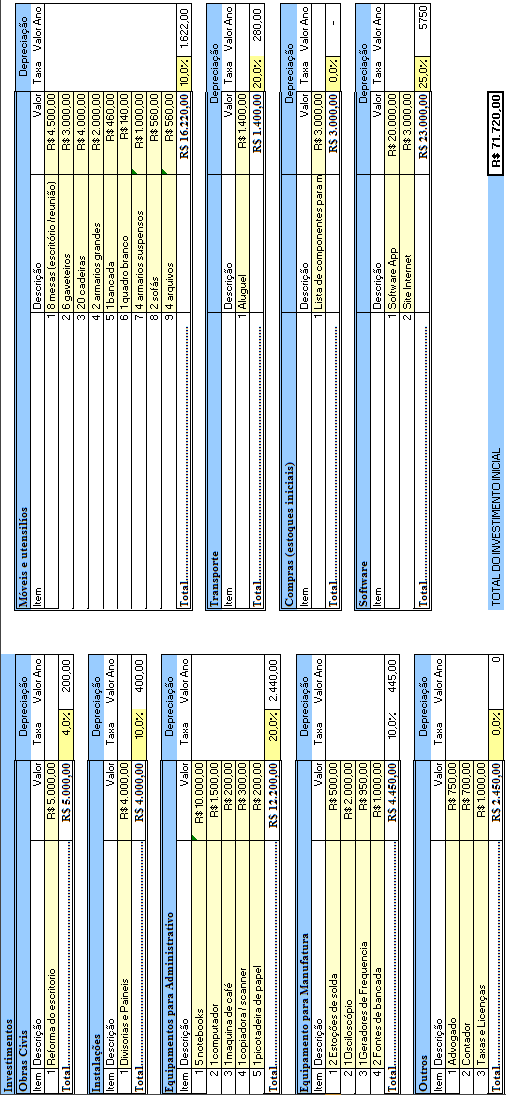
\includegraphics[width=0.55\linewidth]{./figs/inv_inicial}
		
		\begin{small}
			FONTE: Elaborado pelos autores.
		\end{small}
	\end{figure}
	\pagebreak
	
	Feito um levanto com os sócios da empresa, onde foi levantando um capital inicial de R\$ 50.000,00, para arrecadar o montande restante, é necessário um empréstimo bancário, que pode ser viabilizado conforme a Figura \ref{emprestimo}.
	
	\begin{figure}[th]
		\caption{INVESTIMENTO INICIAL DA CUBOBRASIL}
		\label{emprestimo}
		\centering
		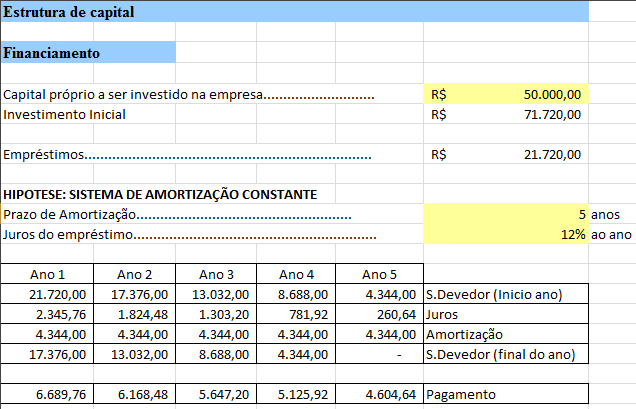
\includegraphics[width=0.8\linewidth]{./figs/emprestimo}
		
		\begin{small}
			FONTE: Elaborado pelos autores.
		\end{small}
	\end{figure}
	\pagebreak

	Com o plano de amortização do empréstimo de R\$ 21.720,00, a CuboBrasil conseguiria pagar todo o empréstimo segundo o plano apresentado na Figura \ref{emprestimo}.
	
	Com os recursos humanos necessários para o funcionamento da empresa, estima-se um custo de R\$ 443.520,00 no primeiro ano de empresa, custo esse baseado na Figura \ref{recuroso_humanos}.
	
	\begin{figure}[th]
		\caption{CUSTO DOS RECURSOS HUMANOS}
		\label{recuroso_humanos}
		\centering
		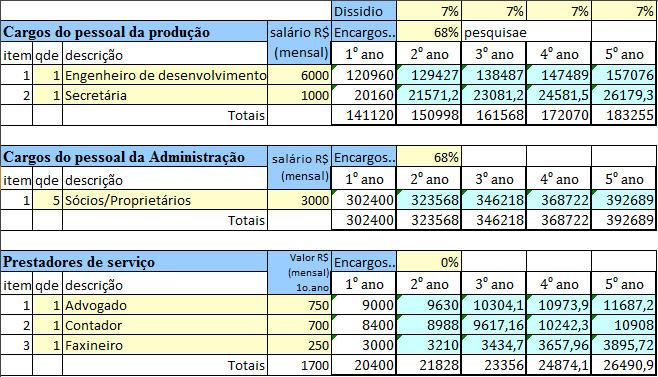
\includegraphics[width=0.8\linewidth]{./figs/recuroso_humanos}
		
		\begin{small}
			FONTE: Elaborado pelos autores.
		\end{small}
	\end{figure}

	Os custos com a operação baseiam-se no descritivo exibido na Figura \ref{operacao}.
	
	\begin{figure}[th]
		\caption{CUSTO COM OPERAÇÃO}
		\label{operacao}
		\centering
		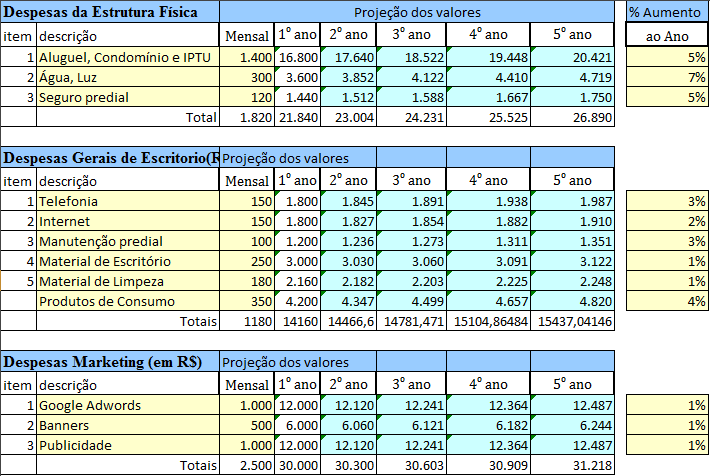
\includegraphics[width=0.8\linewidth]{./figs/operacao}
		
		\begin{small}
			FONTE: Elaborado pelos autores.
		\end{small}
	\end{figure}
	\pagebreak
	
	Para a precificação dos produtos e serviços, foi realizado um levantamento de todos os custos necessários, conforme Figuras \ref{produto1} e \ref{produto2}.

	\begin{figure}[th]
		\caption{PRODUTOS}
		\label{produto1}
		\centering
		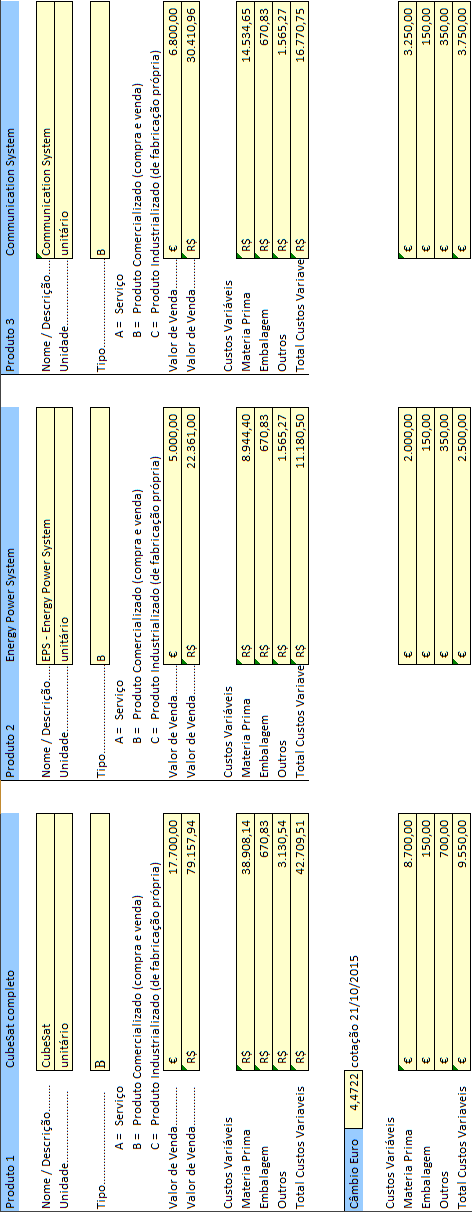
\includegraphics[width=0.45\linewidth]{./figs/produto1}
		
		\begin{small}
			FONTE: Elaborado pelos autores.
		\end{small}
	\end{figure}
	\pagebreak
	
	Nos serviços encontra-se a grande oportunidade de negócio da empresa, uma vez que os custos variáveis praticamente são inexistentes comparados aos custos variáveis dos produtos.
	
	\begin{figure}[th]
		\caption{SERVIÇOS}
		\label{produto2}
		\centering
		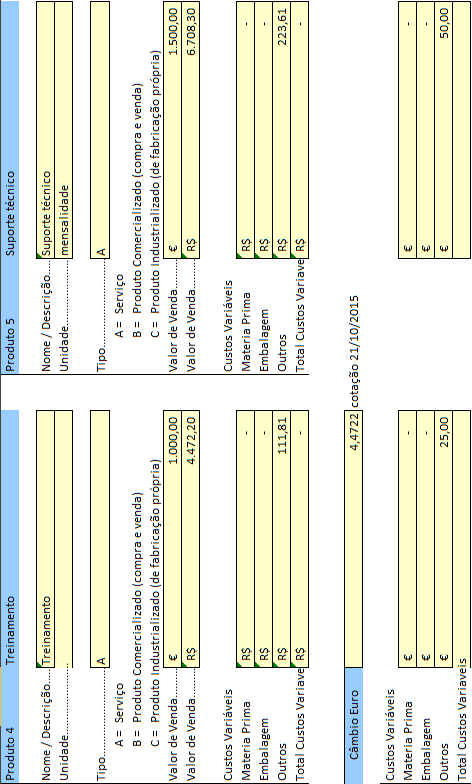
\includegraphics[width=0.6\linewidth]{./figs/produto2}
		
		\begin{small}
			FONTE: Elaborado pelos autores.
		\end{small}
	\end{figure}
	\pagebreak
	
	Em um cenário otimista e não muito fora da realidade, a projeção de vendas da CuboBrasil está representada na Figura \ref{vendas}.
	
	\begin{figure}[th]
		\caption{VENDAS}
		\label{vendas}
		\centering
		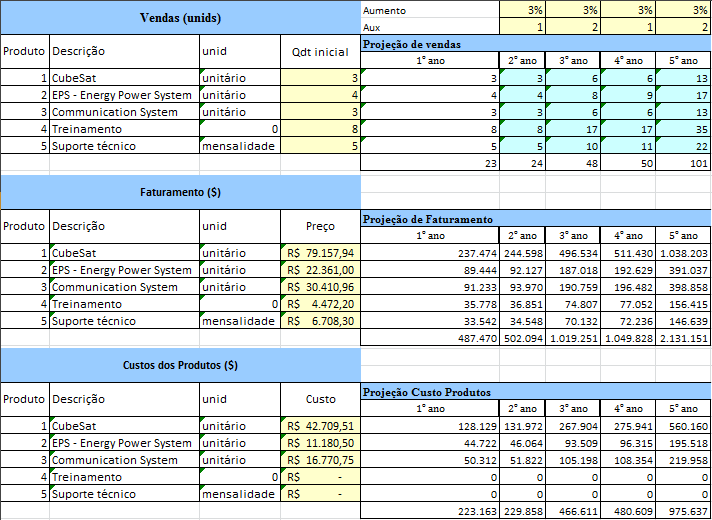
\includegraphics[width=0.8\linewidth]{./figs/vendas}
		
		\begin{small}
			FONTE: Elaborado pelos autores.
		\end{small}
	\end{figure}
	\pagebreak
	
	A CuboBrasil se enquadra na classificação de impostos do Simples nacional, uma vez que seu faturamento anual previsto para até o 5º ano de vida empresa é inferior aos R\$ 2.400.000,00, conforme ilustrado na Figura \ref{simples}.
	
	\begin{figure}[th]
		\caption{TABELA DO SIMPLES NACIONAL}
		\label{simples}
		\centering
		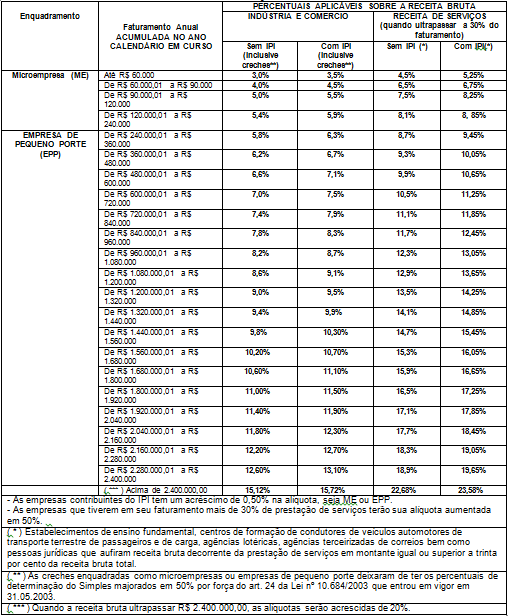
\includegraphics[width=0.8\linewidth]{./figs/simples}
		
		\begin{small}
			FONTE: Editada pelos autores da original disponibilizada pela Receita Federal.
		\end{small}
	\end{figure}
	\pagebreak
	
	Baseado em todo o estudo financeiro da CuboBrasil, obtem-se os resultados expressos na Figura \ref{resultados}.
	
	\begin{figure}[th]
		\caption{PROJEÇÃO DE RESULTADOS}
		\label{resultados}
		\centering
		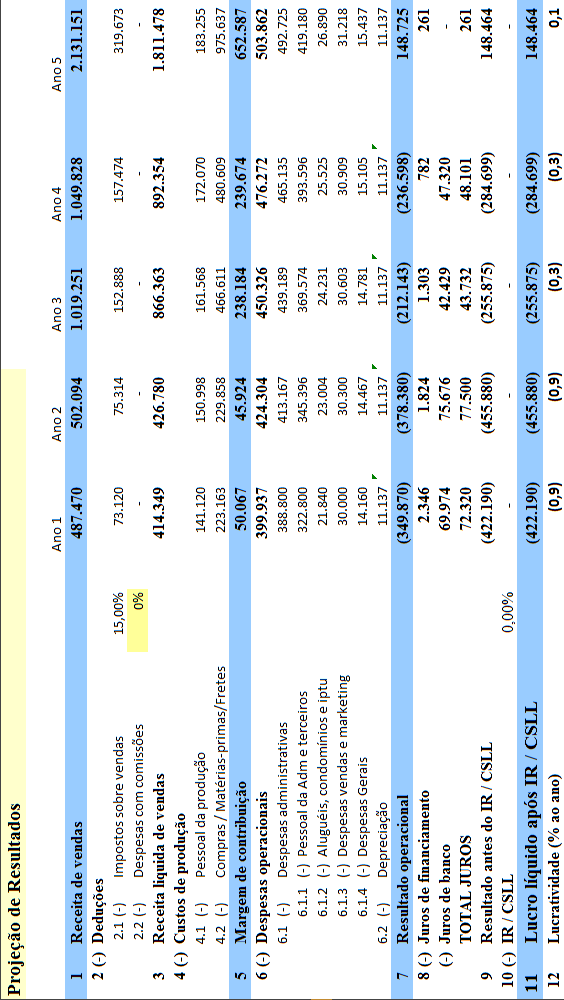
\includegraphics[width=0.6\linewidth]{./figs/resultados}
		
		\begin{small}
			FONTE: Elaborado pelos autores.
		\end{small}
	\end{figure}
	\pagebreak
	
	Analisando o resultado da projeção financeira, é possível verificar que durante os 4 primeiros anos de vida da empresa, a mesma irá trabalhar com um prejuízo total de R\$ 1.418.644,00, para a partir do 5º ano começar a ter um retorno sobre o investimento realizado.
	
	Dessa forma, pode ser concluído que o modelo de negócio proposto para a CuboBrasil, não seja o mais adequado, uma vez que o retorno de todo o investimento feito para iniciar as atividades da empresa irão demorar muito tempo para começar a ter um retorno, que inicialmente será ainda bem abaixo do que o pensado anteriormente a elaboração do plano de negócios da empresa. 
	
	Uma possível forma de garantir a viabilidade do negócio implicaria numa empresa com um planejamento e estrutura muito inferior ao que foi proposto no plano atual, porém esse novo planejamento e estrutura impactariam negativamente na qualidade que a CuboBrasil gostaria de oferecer aos clientes. Para conseguir realizar todo o trabalho proposto nesse plano, a CuboBrasil necessitaria se beneficiar de apoios governamentais ou de possíveis empresas patrocinadoras e de diversas parcerias com instituições respeitas e estivessem dispostas a ajudar a difundir o segmento aeroespacial no Brasil.

% ----------------------------------------------------------
% REFERÊNCIAS BIBLIOGRÁFICAS
% ----------------------------------------------------------
\chapter[Referências bibliográficas]{Referências bibliográficas}

\textbf{Livros:}
	
BRENES, E. R.; MENA, M.; MOLINA, G.E. Key success factors for strategy implementation in Latin America. Journal of Business Research, n. 61, 2011.

BOSSIDY, L.; CHARAN, R. Desafio: fazer acontecer, a disciplina de execução nos negócios. 3ªed. Rio de Janeiro: Negócio Editora, 2002.

HREBINIAK, L.G. Fazendo a estratégia funcionar: o caminho para uma execução bemsucedida. Rio Grande do Sul: Bookman, 2006.

MINTZBERG, H. A criação artesanal da estratégia. In:  Estratégia: a busca da vantagem competitiva. Rio de Janeiro: Campus, 1998. 

OLIVEIRA, Djalma de Pinho Rebouças de. Planejamento estratégico: conceitos, metodologia e praticas. 20 ed. São Paulo: Atlas, 2004.

PEREIRA, Mauricio Fernandes. Planejamento estratégico: teorias, modelos e processo. São Paulo: Atlas, 2011	.
 
SAPIRO, I. C. A. Planejamento Estratégico: Fundamentos e Aplicações. Rio de Janeiro, Elsevier, 2004.

PORTER, M. Vantagem competitiva - Criando e sustentando um desempenho superior. Rio de Janeiro, Elsevier, 1989.

	\textbf{Sites:}
	
	APRENDER. Implementação do planejamento estratégico. Disponível em: \linebreak <http://www.aprendervirtual.com.br/noticiaInterna.php?ID=62\&IDx=113>. Acesso em 05 de mar. 2015.
	
	GUIA DO ESTUDANTE. Marketing. Disponível em: <http://guiadoestudante.abril. com.br/profissoes/adminis tracao-negocios/marketing-686505.shtml>. Acesso em 14 de abr. 2015.
	
	TRT 10 – GESTÃO ESTRATÉGICA. O que é planejamento estratégico. Disponível em: <http://gestaoestrategica.trt10.jus.br/portal/index.php?option=com\_content\&view =article\&id=62:o-que-e-planejamento-estrategico-\&catid=31:general\&Itemid=76>. Acesso em 05 de mar. 2015.
	
	SIGNIFICADOS. O que é marketing. Disponível em: <http://www. significados.com.br/marketing/>. Acesso em 14 de abr. 2015.

	ASSOCIAÇÃO DAS INDÚSTRIAS AEROESPACIAIS DO BRASIL. Números da AIAB. Disponível em: <http://www.aiab.org.br/>. Acesso em 03 de jun. 2015.
	
	ASSOCIAÇÃO DAS INDÚSTRIAS AEROESPACIAIS DO BRASIL. Associadas. Disponível em: <http://www.aiab.org.br/>. Acesso em 03 de jun. 2015.
	
	AGÊNCIA ESPACIAL BRASILEIRA. Instituições firmam convênio para promover indústria aeroespacial. Disponível em: <http://www.aeb.gov.br/instituicoes-firmam-convenio-para-promover-industria-aeroespacial/>. Acesso em 12 de jun. de 2015.
	
	PORTAL ADMINISTRAÇÃO. Análise SWOT (Matriz) - Conceito e aplicação. Disponível em: <http://www.portal-administracao.com/2014/01/analise-swot-conceito-e-aplicacao.html>. Acesso em 11 de jun. de 2015.

	ADMINISTRADORES. Estrutura organizacional - Influência da estrutura na eficiência da organização de acordo. Disponível em: <http://www.administradores.com.br/artigos/\\marketing/estrutura-organizacional-influencia-da-estrutura-na-eficiencia-da-organizacao-de-acordo/62071/>. Acesso em 11 de jun. de 2015.
	
	EXAME. Os salários dos engenheiros no Brasil. Disponível em:\\ <http://exame.abril.com.br/carreira/noticias/quanto-ganham-os-engenheiros-no-brasil>. Acesso em 21 de set. de 2015.
	
	TABELA SALARIAL. Tabela Salarial - Piso Salarial 2015. Disponível em:\\ <http://tabelasalarial.com/consulta-tabela-salarial-2014-atualizada/>. Acesso em 21 de set. de 2015.
	
	ESAG JR. Plano Operacional. Disponível em: <http://esagjr.com.br/plano-operacional/>. Acesso em 21 de set. de 2015.

% ----------------------------------------------------------
% Anexos
% ----------------------------------------------------------

% ---
% Inicia os anexos
% ---
\begin{anexosenv}

% Imprime uma página indicando o início dos anexos
\partanexos

% ---
\chapter{\textit{Business Model} Canvas da CuboBrasil}
% ---
	Modelo Canvas da CuboBrasil, elaborado pelos autores do planejamento estratégico da empresa.
	
	\begin{figure}[th]
		\centering
		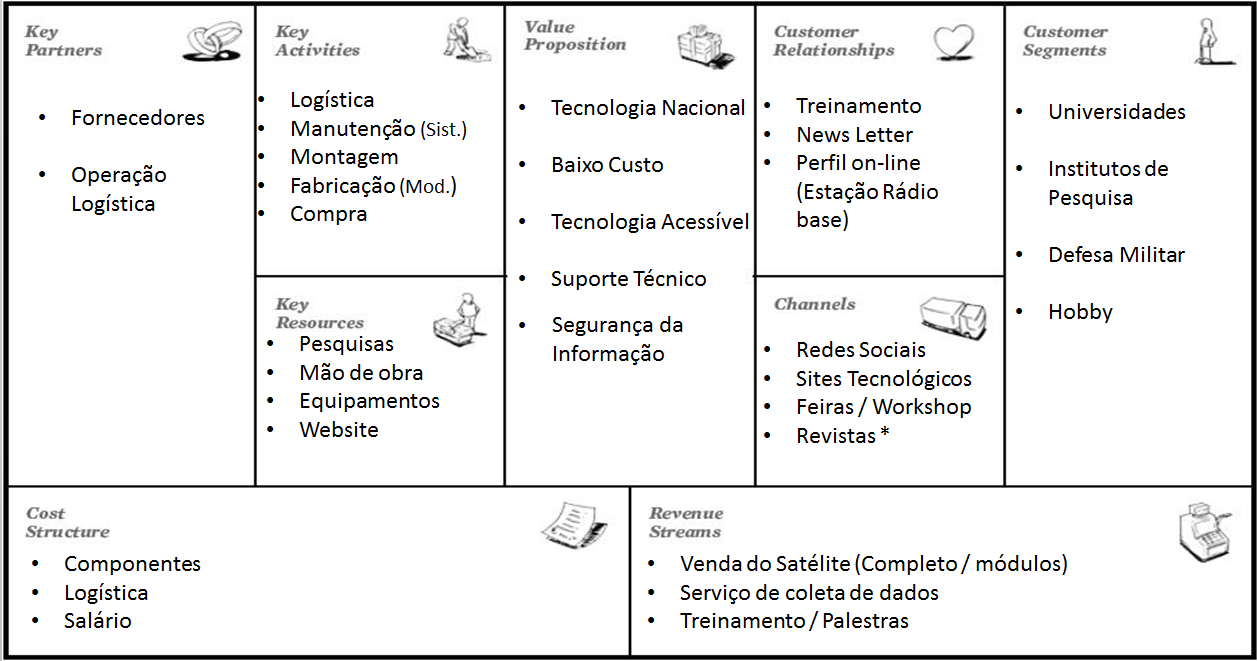
\includegraphics[width=1.0\linewidth]{./figs/Anexo_01}
	\end{figure}

\end{anexosenv}



% ----------------------------------------------------------
% 
% ----------------------------------------------------------
%\chapter[]{}









%---------------------------------------------------------------------
% INDICE REMISSIVO
%---------------------------------------------------------------------
\phantompart
\printindex
%---------------------------------------------------------------------

\end{document}
